
\section*{CHƯƠNG 3. THIẾT KẾ HỆ THỐNG}
\setcounter{section}{3}
\setcounter{subsection}{0} %LƯU Ý MỖI LẦN THÊM CHƯƠNG MỚI CẦN THÊM CÂU NÀY ĐỂ RESET THỨ TỰ CỦA SUBSECTON VỀ 1
\setcounter{table}{0} % LƯU Ý SAU MỖI LẦN GỌI BẢNG HAY HÌNH ẢNH PHẢI THÊM CÂU NÀY ĐỂ RESET THỨ TỰ
\setcounter{figure}{0} %% LƯU Ý SAU MỖI LẦN GỌI BẢNG HAY HÌNH ẢNH PHẢI THÊM CÂU NÀY ĐỂ RESET THỨ TỰ
\addcontentsline{toc}{section}{\numberline{}CHƯƠNG 3. THIẾT KẾ HỆ THỐNG}

Ở chương này, chúng em mô tả quá trình thiết kế hệ thống từ tổng quan đến chi tiết, dựa trên phân tích ở Chương 2.
Mở đầu là xây dựng sơ đồ kiến trúc hệ thống.
Tiếp theo, chương tập trung vào thiết kế giao diện người dùng và các chức năng chính cho website cùng server.
Nội dung chính được thể hiện qua hình ảnh và sơ đồ minh họa, không chỉ mô tả chi tiết luồng hoạt động mà còn làm rõ cách các thành phần trong hệ thống phối hợp, hỗ trợ lẫn nhau.
\subsection{Sơ đồ tổng quan kiến trúc của hệ thống}

\begin{figure}[H]
	\centering
	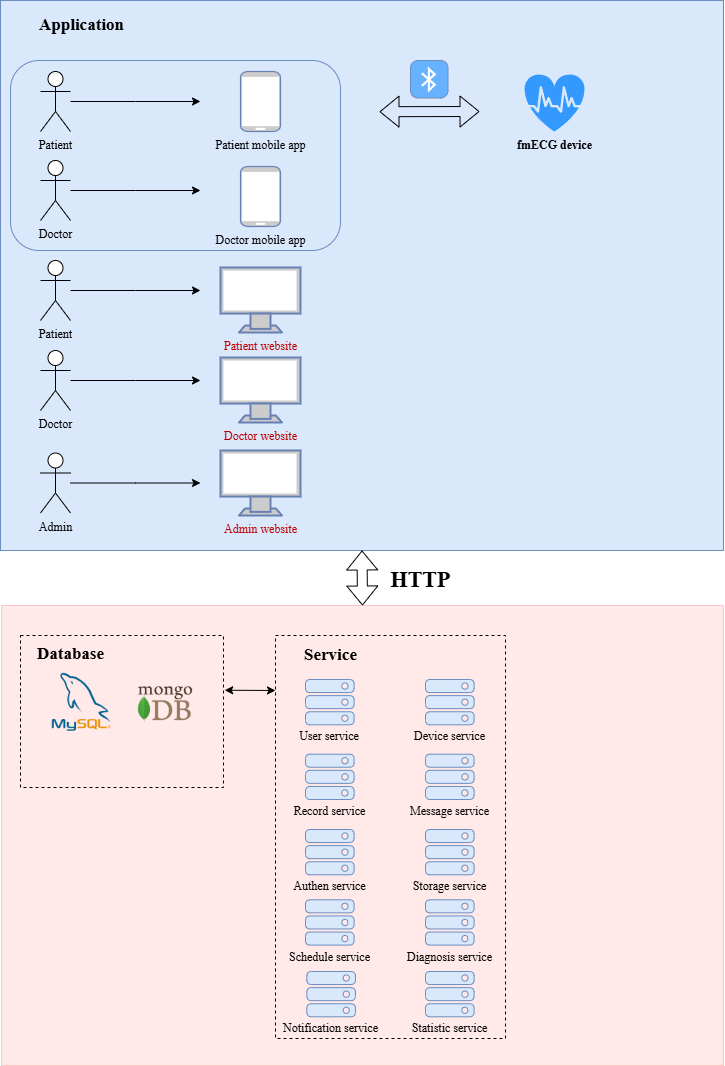
\includegraphics[width=12cm,height=16cm]{Images/System/fmECG_architecture-System_Architecture.drawio.png}
	\caption[Tổng quan kiến trúc hệ thống]{\bfseries \fontsize{12pt}{0pt}\selectfont Tổng quan kiến trúc hệ thống}
	\label{fmECG_architecture-System} %đặt tên cho ảnh
\end{figure}
Hệ thống được chia thành ba phần chính: Thiết bị (Device), Máy chủ (Server) và Ứng dụng (bao gồm web và app).
Mỗi thành phần đảm nhiệm một vai trò quan trọng, cùng phối hợp để đảm bảo hoạt động của toàn bộ hệ thống như được minh họa trong hình vẽ.

Hình \ref{fmECG_architecture-System} thể hiện ba phần:

\begin{adjustwidth}{1.5em}{}
	\begin{itemize}
		\item Device (Thiết bị): Gồm các thiết bị phần cứng đo điện tim, có khả năng kết nối với ứng dụng di động của bệnh nhân thông qua Bluetooth.
		\item Application (Ứng dụng): Bao gồm ứng dụng di động và website, phục vụ nhu cầu sử dụng của bệnh nhân, bác sĩ và quản trị viên.
		\item Server (Máy chủ): Chứa các dịch vụ (Services) xử lý yêu cầu từ ứng dụng và quản lý cơ sở dữ liệu.
	\end{itemize}
\end{adjustwidth}

Trong sơ đồ kiến trúc hệ thống, bệnh nhân sử dụng ứng dụng di động (Mobile App) để kết nối trực tiếp với thiết bị (Device).
Ứng dụng di động thuộc Khối Ứng dụng (Application), chịu trách nhiệm giao tiếp với Khối Máy chủ (Server) thông qua các API và giao thức HTTP.
Khi nhận được yêu cầu từ Application, Server sẽ thực hiện xử lý dữ liệu thông qua các dịch vụ (Services) được thiết kế riêng biệt.
Tùy theo loại yêu cầu, các dịch vụ này sẽ truy xuất hoặc cập nhật dữ liệu trong cơ sở dữ liệu, sau đó gửi kết quả phản hồi cho người dùng,
hoàn thiện quá trình tương tác giữa người dùng và hệ thống.\begin{adjustwidth}{1.5em}{}
	\begin{itemize}
		\item Authen Service: Đảm nhận các nhiệm vụ liên quan đến bảo mật hệ thống, bao gồm mã hóa dữ liệu nhạy cảm, tạo và xác minh token để đảm bảo tính an toàn khi truy cập,
		      quản lý phân quyền người dùng đối với API,và thực hiện mã hóa thông tin trước khi lưu trữ nhằm ngăn chặn rò rỉ dữ liệu.
		\item User Service: Xử lý toàn bộ các thao tác liên quan đến người dùng, như tạo tài khoản mới, xác minh thông tin đăng nhập, lấy thông tin cá nhân của người dùng,
		      đồng thời hỗ trợ cập nhật và chỉnh sửa thông tin cá nhân khi cần thiết.
		\item Device Service: Chịu trách nhiệm quản lý thiết bị, bao gồm các chức năng như thêm mới, chỉnh sửa thông tin, xóa thiết bị,
		      và cập nhật tình trạng thiết bị hoặc thông số liên quan để đảm bảo thiết bị hoạt động đúng trong hệ thống.
		\item Storage Service: Quản lý và vận hành hệ thống lưu trữ dữ liệu, bao gồm lưu trữ file, tài liệu, và các thông tin quan trọng của hệ thống.
		      Đồng thời, đảm bảo tính nhất quán của dữ liệu thông qua cơ chế xử lý race condition, khóa truy cập và đồng bộ hóa dữ liệu trong các trường hợp truy cập đồng thời,
		      cũng như tối ưu hóa hiệu suất lưu trữ và truy xuất dữ liệu.
		\item Record Service: Xử lý các dữ liệu liên quan đến phiên đo, bao gồm thêm mới, cập nhật, xóa dữ liệu, và xử lý các file đo được từ thiết bị trước khi lưu trữ hoặc gửi đến người dùng.
		\item Message Service: Quản lý toàn bộ các yêu cầu liên quan đến nhắn tin, bao gồm gửi, nhận, lưu trữ tin nhắn, hỗ trợ các nhóm trò chuyện giữa những người dùng trong hệ thống.
		\item Schedule Service: Đảm nhiệm việc quản lý lịch khám, bao gồm đặt lịch và xử lý các phản hồi liên quan, nhằm đảm bảo quy trình đặt lịch diễn ra mượt mà giữa bệnh nhân, bác sĩ và hệ thống.
		\item Diagnosis Service: Quản lý các tác vụ liên quan đến chẩn đoán, bao gồm thêm mới và chỉnh sửa thông tin chẩn đoán cho bệnh nhân, đảm bảo dữ liệu chính xác và hỗ trợ quá trình điều trị hiệu quả.
		\item Notification Service: Đảm bảo quản lý hiệu quả các thông báo cho người dùng, từ việc gửi thông báo sự kiện, cảnh báo, đến nhắc nhở,
		      giúp người dùng cập nhật kịp thời các thông tin quan trọng từ hệ thống.
		\item Statistic Service: Chịu trách nhiệm tổng hợp số liệu thống kê trong hệ thống, bao gồm số lượng người dùng (bệnh nhân và bác sĩ),
		      số thiết bị, và dữ liệu phiên đo theo từng tháng, nhằm cung cấp thông tin phục vụ quản lý hiệu quả.
	\end{itemize}
\end{adjustwidth}

Dưới đây là mô tả chi tiết về các phần nhỏ hơn trong kiến trúc hệ thống, được xây dựng dựa trên các đối tượng chính đã phân tích.
\newpage
\subsection{Sơ đồ khối phần mềm}

\subsubsection{Website dành cho bệnh nhân}
\begin{figure}[H]
	\centering
	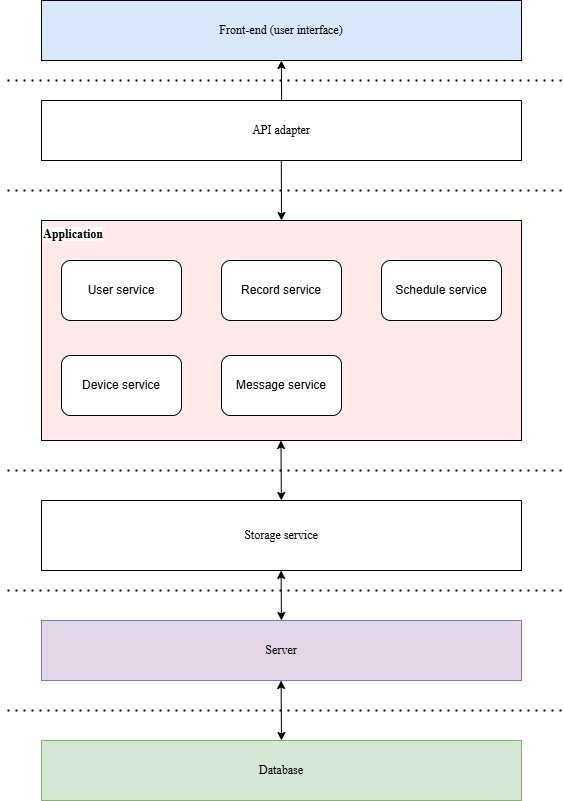
\includegraphics[width=12cm,height=15cm]{Images/System/fmECG_architecture-Patient.drawio.png}
	\caption[Sơ đồ khối Website dành cho bệnh nhân]{\bfseries \fontsize{12pt}{0pt}\selectfont Sơ đồ khối Website dành cho bệnh nhân}
	\label{fmECG_architecture-Patient} %đặt tên cho ảnh
\end{figure}
Tầng trên cùng trong sơ đồ hình \ref{fmECG_architecture-Patient} là User Interface (Giao diện người dùng), nơi bệnh nhân trực tiếp tương tác với hệ thống thông qua API Adapter để gửi yêu cầu và nhận phản hồi.
Các yêu cầu này được xử lý bởi các Services chính, bao gồm User Service, Device Service, Record Service, Schedule Service, Diagnosis Service, Notification Service và Storage Service.

Những Services này được thiết kế nhằm đáp ứng các nhu cầu của bệnh nhân, từ quản lý thông tin cá nhân, mượn và trả thiết bị, theo dõi lịch sử dữ liệu phiên đo, cho đến việc quản lý lịch khám,
tra cứu thông tin chẩn đoán cho từng lịch khám. Ngoài ra, hệ thống còn đảm bảo việc gửi thông báo nhắc nhở kịp thời và hỗ trợ bệnh nhân trao đổi thông tin với bác sĩ một cách liền mạch và hiệu quả.

\subsubsection{Website dành cho bác sĩ}
\begin{figure}[H]
	\centering
	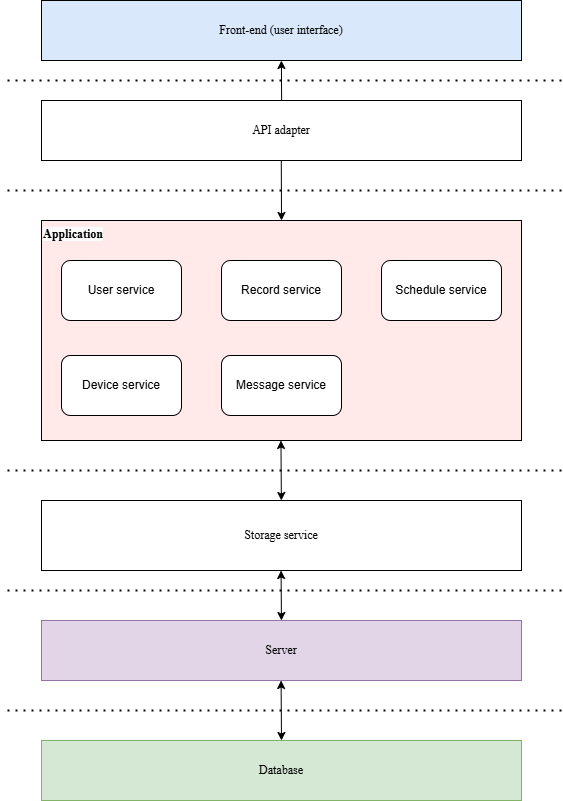
\includegraphics[width=12cm,height=15cm]{Images/System/fmECG_architecture-Doctors.drawio.png}
	\caption[Sơ đồ khối Website dành cho bác sĩ]{\bfseries \fontsize{12pt}{0pt}\selectfont Sơ đồ khối Website dành cho bác sĩ}
	\label{fmECG_architecture-Doctor} %đặt tên cho ảnh
\end{figure}

Tương tự với bệnh nhân, sơ đồ hình \ref{fmECG_architecture-Doctor} được xây dựng để hỗ trợ bác sĩ thực hiện các nhiệm vụ chuyên môn thông qua giao diện người dùng và API Adapter, đảm bảo việc xử lý thông tin diễn ra nhanh chóng và hiệu quả.

Các Services chính, bao gồm User Service, Device Service, Record Service, Schedule Service, Diagnosis Service, Notification Service và Storage Service, đóng vai trò quan trọng trong việc hỗ trợ bác sĩ.
Các nhiệm vụ được tập trung vào việc theo dõi và phân tích dữ liệu phiên đo từ bệnh nhân, quản lý lịch khám, chấp nhận hoặc từ chối yêu cầu đặt lịch, ghi nhận thông tin chẩn đoán, và trao đổi trực tiếp với bệnh nhân.
Hơn nữa, hệ thống cung cấp khả năng tự động gửi thông báo về lịch khám và nhắc nhở các cuộc khám sắp tới, giúp bác sĩ quản lý thời gian và công việc hiệu quả hơn.

Cách tiếp cận này không chỉ hỗ trợ bác sĩ tổ chức công việc thuận lợi mà còn góp phần nâng cao hiệu quả điều trị cho bệnh nhân.

\subsubsection{Website cho quản trị viên}
\begin{figure}[H]
	\centering
	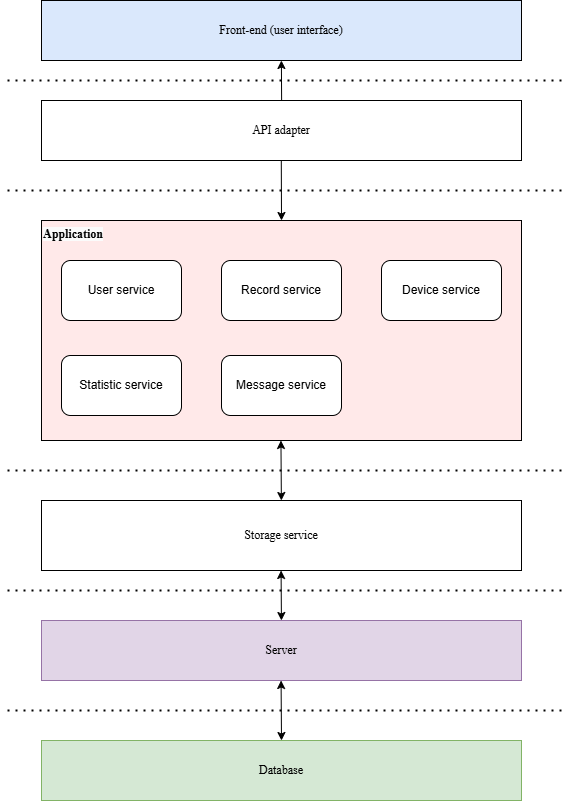
\includegraphics[width=12cm,height=15cm]{Images/System/fmECG_architecture-Admin.drawio.png}
	\caption[Sơ đồ khối Website dành cho quản trị viên]{\bfseries \fontsize{12pt}{0pt}\selectfont Sơ đồ khối Website dành cho quản trị viên}
	\label{fmECG_architecture-Admin} %đặt tên cho ảnh
\end{figure}
Về cơ bản, website dành cho admin được thiết kế với cấu trúc tương tự như website dành cho bác sĩ và bệnh nhân nhưng với quyền hạn mở rộng hơn.
Admin có thể quản lý toàn bộ thông tin người dùng, dữ liệu phiên đo, theo dõi các thống kê tổng quan của hệ thống, kiểm soát thông tin và kết quả chẩn đoán từ các lịch khám,
đồng thời điều hành việc mượn trả thiết bị một cách linh hoạt và hiệu quả.

\subsection{Thiết kế cơ sở dữ liệu}

\subsubsection{Chuyển đổi từ mô hình thực thể liên kết sang mô hình quan hệ}
Dựa trên bảng mô tả các thực thể và thuộc tính, chúng em tiến hành chuyển đổi từ mô hình thực thể liên kết thành mô hình quan hệ như sau.

\begin{itemize}
	\item Tài khoản đăng nhập (\textbf{ID tài khoản đăng nhập}, Địa chỉ email đăng ký, Mật khẩu truy cập)
	\item Token đăng nhập (\textbf{ID token đăng nhập}, ID tài khoản đăng nhập, Token làm mới, Hạn sử dụng, Trạng thái token)
	\item Vai trò người dùng (\textbf{ID vai trò}, Tên vai trò)
	\item Trạng thái hoạt động (\textbf{ID trạng thái người dùng}, Mô tả trạng thái người dùng)
	\item Người dùng (\textbf{ID người dùng}, ID tài khoản đăng nhập, ID vai trò người dùng, ID trạng thái hoạt động, Tên đầy đủ, Ngày tháng năm sinh, Giới tính, Số liên lạc, Đường dẫn ảnh đại diện, Thông tin bổ sung)
	\item Loại thiết bị (\textbf{ID loại thiết bị}, Tên loại thiết bị)
	\item Trạng thái thiết bị (\textbf{ID trạng thái thiết bị}, Mô tả trạng thái thiết bị)
	\item Thiết bị (\textbf{ID thiết bị}, ID người dùng thiết bị, ID loại thiết bị, ID trạng thái thiết bị, Tên thiết bị, Thông tin chi tiết về thiết bị, Ngày bắt đầu thời gian mượn, Ngày kết thúc thời gian mượn)
	\item Thông số kỹ thuật (\textbf{ID thông số kỹ thuật}, ID thiết bị, Loại thông số, Tên thông số, Giá trị thông số, Mô tả chi tiết thông số)
	\item Dữ liệu phiên đo (\textbf{ID dữ liệu phiên đo}, ID bệnh nhân, ID thiết bị, Loại bản ghi, Đường dẫn lưu trữ dữ liệu phiên đo, Thời gian bắt đầu thu thập dữ liệu, Thời gian kết thúc thu thập dữ liệu)
	\item Trạng thái lịch khám (\textbf{ID trạng thái lịch khám}, Mô tả trạng thái lịch khám)
	\item Kết quả lịch khám (\textbf{ID kết quả lịch khám}, Mô tả kết quả lịch khám)
	\item Lịch khám (\textbf{ID lịch khám}, ID bệnh nhân, ID bác sĩ, ID trạng thái lịch khám, ID kết quả lịch khám, Thời gian bắt đầu lịch khám, Thời gian kết thúc lịch khám)
	\item Thông báo liên quan đến lịch khám (\textbf{ID thông báo}, ID lịch khám, Loại thông báo, Nội dung thông báo, Trạng thái thông báo, Trạng thái đã xem, Lý do từ chối lịch khám)
	\item Chẩn đoán (\textbf{ID chẩn đoán}, ID lịch khám, Thông tin chẩn đoán)
	\item Tin nhắn (\textbf{ID tin nhắn}, ID người gửi, ID nhóm trò chuyện nhận tin nhắn, Nội dung tin nhắn, Thời gian gửi tin nhắn)
	\item Nhóm trò chuyện (\textbf{ID nhóm trò chuyện}, Tên nhóm trò chuyện, Người tạo nhóm, Danh sách thành viên nhóm, Sự kiện gửi tin nhắn, Sự kiện nhận tin nhắn)

\end{itemize}

\subsubsection{Chuẩn hoá 3NF}
Các bảng đã được thiết kế theo nguyên tắc chuẩn hoá 3NF, vì không có thuộc tính lặp lại và các thuộc tính không phụ thuộc vào một tập hợp con của khóa chính.

\paragraph{Chuẩn hoá bảng Tài khoản}
\mbox{}
\begin{table}[H]
	\caption{\bfseries \fontsize{12pt}{0pt}\selectfont Bảng chuẩn hoá bảng Tài khoản đăng nhập}
	\centering
	\begin{tabularx}{0.9\textwidth}{|X|X|}
		\hline
		\textbf{Danh sách thuộc tính} & ID tài khoản đăng nhập, Địa chỉ email đăng ký, Mật khẩu truy cập                                   \\
		\hline
		\textbf{Quy tắc nghiệp vụ}    & \textbf{Phụ thuộc hàm}                                                                             \\
		\hline
		Mỗi tài khoản có một ID riêng, có duy nhất Địa chỉ email đăng ký, Mật khẩu truy cập
		                              & \parbox[t]{\linewidth}{$\text{ID tài khoản} \rightarrow$ Địa chỉ email đăng ký, Mật khẩu truy cập} \\
		\hline
		\multicolumn{2}{|X|}{$\Rightarrow \text{Khoá chính của bảng: ID tài khoản đăng nhập}$}                                             \\
		\multicolumn{2}{|X|}{$\Rightarrow \text{Bảng Tài khoản đăng nhập đã ở 3NF}$}                                                       \\
		\hline
	\end{tabularx}
\end{table}

\paragraph{Chuẩn hoá bảng Token đăng nhập}
\mbox{}
\begin{table}[H]
	\caption{\bfseries \fontsize{12pt}{0pt}\selectfont Bảng chuẩn hoá bảng Token đăng nhập}
	\centering
	\begin{tabularx}{0.9\textwidth}{|X|X|}
		\hline
		\textbf{Danh sách thuộc tính} & ID token đăng nhập, ID tài khoản đăng nhập, Token làm mới, Hạn sử dụng, Trạng thái token                         \\
		\hline
		\textbf{Quy tắc nghiệp vụ}    & \textbf{Phụ thuộc hàm}                                                                                           \\
		\hline
		Mỗi tài khoản có một ID token riêng, có duy nhất ID tài khoản, Token làm mới, Hạn sử dụng, Trạng thái token
		                              & \parbox[t]{\linewidth}{$\text{ID token} \rightarrow$ ID tài khoản, Token làm mới, Hạn sử dụng, Trạng thái token} \\
		\hline
		\multicolumn{2}{|X|}{$\Rightarrow \text{Khoá chính của bảng: ID token đăng nhập}$}                                                               \\
		\multicolumn{2}{|X|}{$\Rightarrow \text{Bảng Token đăng nhập đã ở 3NF}$}                                                                         \\
		\hline
	\end{tabularx}
\end{table}

\paragraph{Chuẩn hoá bảng Vai trò người dùng}
\mbox{}
\begin{table}[H]
	\caption{\bfseries \fontsize{12pt}{0pt}\selectfont Bảng chuẩn hoá bảng Vai trò người dùng}
	\centering
	\begin{tabularx}{0.9\textwidth}{|X|X|}
		\hline
		\textbf{Danh sách thuộc tính} & ID vai trò, Tên vai trò                                             \\
		\hline
		\textbf{Quy tắc nghiệp vụ}    & \textbf{Phụ thuộc hàm}                                              \\
		\hline
		Mỗi vai trò có một ID riêng, có duy nhất Tên vai trò
		                              & \parbox[t]{\linewidth}{$\text{ID vai trò} \rightarrow$ Tên vai trò} \\
		\hline
		\multicolumn{2}{|X|}{$\Rightarrow \text{Khoá chính của bảng: ID vai trò}$}                          \\
		\multicolumn{2}{|X|}{$\Rightarrow \text{Bảng Vai trò người dùng đã ở 3NF}$}                         \\
		\hline
	\end{tabularx}
\end{table}

\paragraph{Chuẩn hoá bảng Trạng thái hoạt động}
\mbox{}
\begin{table}[H]
	\caption{\bfseries \fontsize{12pt}{0pt}\selectfont Bảng chuẩn hoá bảng Trạng thái hoạt động}
	\centering
	\begin{tabularx}{0.9\textwidth}{|X|X|}
		\hline
		\textbf{Danh sách thuộc tính} & ID trạng thái người dùng, Mô tả trạng thái người dùng                                             \\
		\hline
		\textbf{Quy tắc nghiệp vụ}    & \textbf{Phụ thuộc hàm}                                                                            \\
		\hline
		Mỗi trạng thái người dùng có một ID riêng, có duy nhất Mô tả trạng thái người dùng
		                              & \parbox[t]{\linewidth}{$\text{ID trạng thái người dùng} \rightarrow$ Mô tả trạng thái người dùng} \\
		\hline
		\multicolumn{2}{|X|}{$\Rightarrow \text{Khoá chính của bảng: ID trạng thái người dùng}$}                                          \\
		\multicolumn{2}{|X|}{$\Rightarrow \text{Bảng Trạng thái hoạt động đã ở 3NF}$}                                                     \\
		\hline
	\end{tabularx}
\end{table}

\paragraph{Chuẩn hoá bảng Người dùng}
\mbox{}
\begin{table}[H]
	\caption{\bfseries \fontsize{12pt}{0pt}\selectfont Bảng chuẩn hoá bảng Người dùng}
	\centering
	\begin{tabularx}{0.9\textwidth}{|X|X|}
		\hline
		\textbf{Danh sách thuộc tính}                                                                                                                                                                                          & ID người dùng, ID tài khoản đăng nhập, ID vai trò người dùng, ID trạng thái hoạt động, Tên đầy đủ, Ngày tháng năm sinh, Giới tính, Số liên lạc, Đường dẫn ảnh đại diện, Thông tin bổ sung                                             \\
		\hline
		\textbf{Quy tắc nghiệp vụ}                                                                                                                                                                                             & \textbf{Phụ thuộc hàm}                                                                                                                                                                                                                \\
		\hline
		Mỗi người dùng có một ID riêng, có duy nhất ID tài khoản đăng nhập, ID vai trò người dùng, ID trạng thái hoạt động, Tên đầy đủ, Ngày tháng năm sinh, Giới tính, Số liên lạc, Đường dẫn ảnh đại diện, Thông tin bổ sung & \parbox[t]{\linewidth}{$\text{ID người dùng} \rightarrow$ ID tài khoản đăng nhập, ID vai trò người dùng, ID trạng thái hoạt động, Tên đầy đủ, Ngày tháng năm sinh, Giới tính, Số liên lạc, Đường dẫn ảnh đại diện, Thông tin bổ sung} \\
		\hline
		\multicolumn{2}{|X|}{$\Rightarrow \text{Khoá chính của bảng: ID người dùng}$}                                                                                                                                                                                                                                                                                                                                                                                  \\
		\multicolumn{2}{|X|}{$\Rightarrow \text{Bảng Người dùng đã ở 3NF}$}                                                                                                                                                                                                                                                                                                                                                                                            \\
		\hline
	\end{tabularx}
\end{table}

\paragraph{Chuẩn hoá bảng Loại thiết bị}
\mbox{}
\begin{table}[H]
	\caption{\bfseries \fontsize{12pt}{0pt}\selectfont Bảng chuẩn hoá bảng Loại thiết bị}
	\centering
	\begin{tabularx}{0.9\textwidth}{|X|X|}
		\hline
		\textbf{Danh sách thuộc tính} & ID loại thiết bị, Tên loại thiết bị                                             \\
		\hline
		\textbf{Quy tắc nghiệp vụ}    & \textbf{Phụ thuộc hàm}                                                          \\
		\hline
		Mỗi loại thiết bị có một ID riêng, có duy nhất Tên loại thiết bị
		                              & \parbox[t]{\linewidth}{$\text{ID loại thiết bị} \rightarrow$ Tên loại thiết bị} \\
		\hline
		\multicolumn{2}{|X|}{$\Rightarrow \text{Khoá chính của bảng: ID loại thiết bị}$}                                \\
		\multicolumn{2}{|X|}{$\Rightarrow \text{Bảng loại thiết bị đã ở 3NF}$}                                          \\
		\hline
	\end{tabularx}
\end{table}

\paragraph{Chuẩn hoá bảng Trạng thái thiết bị}
\mbox{}
\begin{table}[H]
	\caption{\bfseries \fontsize{12pt}{0pt}\selectfont Bảng chuẩn hoá bảng Trạng thái thiết bị}
	\centering
	\begin{tabularx}{0.9\textwidth}{|X|X|}
		\hline
		\textbf{Danh sách thuộc tính} & ID trạng thái thiết bị, Mô tả trạng thái thiết bị                                             \\
		\hline
		\textbf{Quy tắc nghiệp vụ}    & \textbf{Phụ thuộc hàm}                                                                        \\
		\hline
		Mỗi trạng thái thiết bị có một ID riêng, có duy nhất Mô tả trạng thái thiết bị
		                              & \parbox[t]{\linewidth}{$\text{ID trạng thái thiết bị} \rightarrow$ Mô tả trạng thái thiết bị} \\
		\hline
		\multicolumn{2}{|X|}{$\Rightarrow \text{Khoá chính của bảng: ID trạng thái thiết bị}$}                                        \\
		\multicolumn{2}{|X|}{$\Rightarrow \text{Bảng Trạng thái thiết bị đã ở 3NF}$}                                                  \\
		\hline
	\end{tabularx}
\end{table}

\paragraph{Chuẩn hoá bảng Thiết bị}
\mbox{}
\begin{table}[H]
	\caption{\bfseries \fontsize{12pt}{0pt}\selectfont Bảng chuẩn hoá bảng Thiết bị}
	\centering
	\begin{tabularx}{0.9\textwidth}{|X|X|}
		\hline
		\textbf{Danh sách thuộc tính} & ID thiết bị, ID người dùng thiết bị, Tên thiết bị, Thông tin chi tiết về thiết bị, Ngày bắt đầu thời gian mượn, Ngày kết thúc thời gian mượn \\
		\hline
		\textbf{Quy tắc nghiệp vụ}    & \textbf{Phụ thuộc hàm}                                                                                                                       \\
		\hline
		Mỗi thiết bị có một ID thiết bị riêng, có duy nhất tên thiết bị, loại thiết bị, thông tin thiết bị,
		ID người dùng thiết bị, trạng thái thiết bị, ngày bắt đầu sử dụng, ngày kết thúc sử dụng
		                              & \parbox[t]{\linewidth}{$\text{ID thiết bị} \rightarrow$ ID người dùng thiết bị, Tên thiết bị,
		Loại thiết bị, Thông tin thiết bị, Trạng thái thiết bị, Ngày bắt đầu sử dụng, Ngày kết thúc sử dụng}                                                                         \\
		\hline
		\multicolumn{2}{|X|}{$\Rightarrow \text{Khoá chính của bảng: ID thiết bị}$}                                                                                                  \\
		\multicolumn{2}{|X|}{$\Rightarrow \text{Bảng Thiết bị đã ở 3NF}$}                                                                                                            \\
		\hline
	\end{tabularx}
\end{table}

\paragraph{Chuẩn hoá bảng Thông số kỹ thuật}
\mbox{}
\begin{table}[H]
	\caption{\bfseries \fontsize{12pt}{0pt}\selectfont Bảng chuẩn hoá bảng Thông số kỹ thuật}
	\centering
	\begin{tabularx}{0.9\textwidth}{|X|X|}
		\hline
		\textbf{Danh sách thuộc tính} & ID thông số kỹ thuật, ID thiết bị, Loại thông số, Tên thông số, Giá trị thông số, Mô tả chi tiết thông số                                             \\
		\hline
		\textbf{Quy tắc nghiệp vụ}    & \textbf{Phụ thuộc hàm}                                                                                                                                \\
		\hline
		Mỗi thông số kỹ thuật sẽ có một ID riêng, có duy nhất ID thiết bị, Loại thông số, Tên thông số, Giá trị thông số, Mô tả chi tiết thông số
		                              & \parbox[t]{\linewidth}{$\text{ID thông số kỹ thuật} \rightarrow$ ID thiết bị, Loại thông số, Tên thông số, Giá trị thông số, Mô tả chi tiết thông số} \\
		\hline
		\multicolumn{2}{|X|}{$\Rightarrow \text{Khoá chính của bảng: ID thông số kỹ thuật}$}                                                                                                  \\
		\multicolumn{2}{|X|}{$\Rightarrow \text{Bảng Thông số kỹ thuật đã ở 3NF}$}                                                                                                            \\
		\hline
	\end{tabularx}
\end{table}

\paragraph{Chuẩn hoá bảng Dữ liệu phiên đo}
\mbox{}
\begin{table}[H]
	\caption{\bfseries \fontsize{12pt}{0pt}\selectfont Bảng chuẩn hoá bảng Dữ liệu phiên đo}
	\centering
	\begin{tabularx}{0.9\textwidth}{|X|X|}
		\hline
		\textbf{Danh sách thuộc tính} & ID dữ liệu phiên đo, ID bệnh nhân, ID thiết bị, Loại bản ghi, Đường dẫn lưu trữ dữ liệu phiên đo, Thời gian bắt đầu thu thập dữ liệu, Thời gian kết thúc thu thập dữ liệu                                             \\
		\hline
		\textbf{Quy tắc nghiệp vụ}    & \textbf{Phụ thuộc hàm}                                                                                                                                                                                                \\
		\hline
		Mỗi dữ liệu phiên đo có một ID riêng, có duy nhất ID bệnh nhân, ID thiết bị, Loại bản ghi, Đường dẫn lưu trữ dữ liệu phiên đo, Thời gian bắt đầu thu thập dữ liệu, Thời gian kết thúc thu thập dữ liệu
		                              & \parbox[t]{\linewidth}{$\text{ID dữ liệu phiên đo} \rightarrow$ ID bệnh nhân, ID thiết bị, Loại bản ghi, Đường dẫn lưu trữ dữ liệu phiên đo, Thời gian bắt đầu thu thập dữ liệu, Thời gian kết thúc thu thập dữ liệu} \\
		\hline
		\multicolumn{2}{|X|}{$\Rightarrow \text{Khoá chính của bảng: ID dữ liệu phiên đo}$}                                                                                                                                                                   \\
		\multicolumn{2}{|X|}{$\Rightarrow \text{Bảng Dữ liệu phiên đo đã ở 3NF}$}                                                                                                                                                                             \\
		\hline
	\end{tabularx}
\end{table}

\paragraph{Chuẩn hoá bảng Trạng thái lịch khám}
\mbox{}
\begin{table}[H]
	\caption{\bfseries \fontsize{12pt}{0pt}\selectfont Bảng chuẩn hoá bảng Trạng thái lịch khám}
	\centering
	\begin{tabularx}{0.9\textwidth}{|X|X|}
		\hline
		\textbf{Danh sách thuộc tính} & ID trạng thái lịch khám, Mô tả trạng thái lịch khám                                             \\
		\hline
		\textbf{Quy tắc nghiệp vụ}    & \textbf{Phụ thuộc hàm}                                                                          \\
		\hline
		Mỗi trạng thái lịch khám có một ID riêng, có duy nhất Mô tả trạng thái lịch khám
		                              & \parbox[t]{\linewidth}{$\text{ID trạng thái lịch khám} \rightarrow$ Mô tả trạng thái lịch khám} \\
		\hline
		\multicolumn{2}{|X|}{$\Rightarrow \text{Khoá chính của bảng: ID trạng thái lịch khám}$}                                         \\
		\multicolumn{2}{|X|}{$\Rightarrow \text{Bảng Trạng thái lịch khám đã ở 3NF}$}                                                   \\
		\hline
	\end{tabularx}
\end{table}

\paragraph{Chuẩn hoá bảng Kết quả lịch khám}
\mbox{}
\begin{table}[H]
	\caption{\bfseries \fontsize{12pt}{0pt}\selectfont Bảng chuẩn hoá bảng Kết quả lịch khám}
	\centering
	\begin{tabularx}{0.9\textwidth}{|X|X|}
		\hline
		\textbf{Danh sách thuộc tính} & ID kết quả lịch khám, Mô tả kết quả lịch khám                                             \\
		\hline
		\textbf{Quy tắc nghiệp vụ}    & \textbf{Phụ thuộc hàm}                                                                    \\
		\hline
		Mỗi Kết quả lịch khám có một ID riêng, có duy nhất Mô tả kết quả lịch khám
		                              & \parbox[t]{\linewidth}{$\text{ID kết quả lịch khám} \rightarrow$ Mô tả kết quả lịch khám} \\
		\hline
		\multicolumn{2}{|X|}{$\Rightarrow \text{Khoá chính của bảng: ID kết quả lịch khám}$}                                      \\
		\multicolumn{2}{|X|}{$\Rightarrow \text{Bảng Kết quả lịch khám đã ở 3NF}$}                                                \\
		\hline
	\end{tabularx}
\end{table}

\paragraph{Chuẩn hoá bảng Lịch khám}
\mbox{}
\begin{table}[H]
	\caption{\bfseries \fontsize{12pt}{0pt}\selectfont Bảng chuẩn hoá bảng Lịch khám}
	\centering
	\begin{tabularx}{0.9\textwidth}{|X|X|}
		\hline
		\textbf{Danh sách thuộc tính} & ID lịch khám, ID bệnh nhân, ID bác sĩ, ID trạng thái lịch khám, ID kết quả lịch khám, Thời gian bắt đầu lịch khám, Thời gian kết thúc lịch khám                                             \\
		\hline
		\textbf{Quy tắc nghiệp vụ}    & \textbf{Phụ thuộc hàm}                                                                                                                                                                      \\
		\hline
		Mỗi Lịch khám có một ID riêng, có duy nhất ID bệnh nhân, ID bác sĩ, ID trạng thái lịch khám, ID kết quả lịch khám, Thời gian bắt đầu lịch khám, Thời gian kết thúc lịch khám
		                              & \parbox[t]{\linewidth}{$\text{ID lịch khám} \rightarrow$ ID bệnh nhân, ID bác sĩ, ID trạng thái lịch khám, ID kết quả lịch khám, Thời gian bắt đầu lịch khám, Thời gian kết thúc lịch khám} \\
		\hline
		\multicolumn{2}{|X|}{$\Rightarrow \text{Khoá chính của bảng: ID  lịch khám}$}                                                                                                                                               \\
		\multicolumn{2}{|X|}{$\Rightarrow \text{Bảng Lịch khám đã ở 3NF}$}                                                                                                                                                          \\
		\hline
	\end{tabularx}
\end{table}

\paragraph{Chuẩn hoá bảng Thông báo liên quan đến lịch khám}
\mbox{}
\begin{table}[H]
	\caption{\bfseries \fontsize{12pt}{0pt}\selectfont Bảng chuẩn hoá bảng Thông báo liên quan đến lịch khám}
	\centering
	\begin{tabularx}{0.9\textwidth}{|X|X|}
		\hline
		\textbf{Danh sách thuộc tính} & ID thông báo, ID lịch khám, Loại thông báo, Nội dung thông báo, Trạng thái thông báo, Trạng thái đã xem, Lý do từ chối lịch khám                                             \\
		\hline
		\textbf{Quy tắc nghiệp vụ}    & \textbf{Phụ thuộc hàm}                                                                                                                                                       \\
		\hline
		Mỗi Thông báo liên quan đến lịch khám có một ID riêng, có duy nhất ID lịch khám, Loại thông báo, Nội dung thông báo, Trạng thái thông báo, Trạng thái đã xem, Lý do từ chối lịch khám
		                              & \parbox[t]{\linewidth}{$\text{ID thông báo} \rightarrow$ ID lịch khám, Loại thông báo, Nội dung thông báo, Trạng thái thông báo, Trạng thái đã xem, Lý do từ chối lịch khám} \\
		\hline
		\multicolumn{2}{|X|}{$\Rightarrow \text{Khoá chính của bảng: ID  thông báo}$}                                                                                                                                \\
		\multicolumn{2}{|X|}{$\Rightarrow \text{Bảng Thông báo liên quan đến lịch khám đã ở 3NF}$}                                                                                                                   \\
		\hline
	\end{tabularx}
\end{table}

\paragraph{Chuẩn hoá bảng Chẩn đoán}
\mbox{}
\begin{table}[H]
	\caption{\bfseries \fontsize{12pt}{0pt}\selectfont Bảng chuẩn hoá bảng Chẩn đoán}
	\centering
	\begin{tabularx}{0.9\textwidth}{|X|X|}
		\hline
		\textbf{Danh sách thuộc tính} & ID chẩn đoán, ID lịch khám, Thông tin chẩn đoán                                             \\
		\hline
		\textbf{Quy tắc nghiệp vụ}    & \textbf{Phụ thuộc hàm}                                                                      \\
		\hline
		Mỗi Chẩn đoán có một ID riêng, có duy nhất ID lịch khám, Thông tin chẩn đoán
		                              & \parbox[t]{\linewidth}{$\text{ID chẩn đoán} \rightarrow$ ID lịch khám, Thông tin chẩn đoán} \\
		\hline
		\multicolumn{2}{|X|}{$\Rightarrow \text{Khoá chính của bảng: ID  chẩn đoán}$}                                               \\
		\multicolumn{2}{|X|}{$\Rightarrow \text{Bảng Chẩn đoán đã ở 3NF}$}                                                          \\
		\hline
	\end{tabularx}
\end{table}

\paragraph{Chuẩn hoá bảng Tin nhắn}
\mbox{}
\begin{table}[H]
	\caption{\bfseries \fontsize{12pt}{0pt}\selectfont Bảng chuẩn hoá bảng Tin nhắn}
	\centering
	\begin{tabularx}{0.9\textwidth}{|X|X|}
		\hline
		\textbf{Danh sách thuộc tính} & ID tin nhắn, ID người gửi, ID nhóm trò chuyện nhận tin nhắn, Nội dung tin nhắn, Thời gian gửi tin nhắn                                             \\
		\hline
		\textbf{Quy tắc nghiệp vụ}    & \textbf{Phụ thuộc hàm}                                                                                                                             \\
		\hline
		Mỗi Tin nhắn có một ID riêng, có duy nhất ID người gửi, ID nhóm trò chuyện nhận tin nhắn, Nội dung tin nhắn, Thời gian gửi tin nhắn
		                              & \parbox[t]{\linewidth}{$\text{ID tin nhắn} \rightarrow$ ID người gửi, ID nhóm trò chuyện nhận tin nhắn, Nội dung tin nhắn, Thời gian gửi tin nhắn} \\
		\hline
		\multicolumn{2}{|X|}{$\Rightarrow \text{Khoá chính của bảng: ID  tin nhắn}$}                                                                                                       \\
		\multicolumn{2}{|X|}{$\Rightarrow \text{Bảng Tin nhắn đã ở 3NF}$}                                                                                                                  \\
		\hline
	\end{tabularx}
\end{table}

\paragraph{Chuẩn hoá bảng Nhóm trò chuyện}
\mbox{}
\begin{table}[H]
	\caption{\bfseries \fontsize{12pt}{0pt}\selectfont Bảng chuẩn hoá bảng Nhóm trò chuyện}
	\centering
	\begin{tabularx}{0.9\textwidth}{|X|X|}
		\hline
		\textbf{Danh sách thuộc tính} & ID nhóm trò chuyện, Tên nhóm trò chuyện, Người tạo nhóm, Danh sách thành viên nhóm, Sự kiện gửi tin nhắn, Sự kiện nhận tin nhắn                                             \\
		\hline
		\textbf{Quy tắc nghiệp vụ}    & \textbf{Phụ thuộc hàm}                                                                                                                                                      \\
		\hline
		Mỗi Nhóm trò chuyện có một ID riêng, có duy nhất Tên nhóm trò chuyện, Người tạo nhóm, Danh sách thành viên nhóm, Sự kiện gửi tin nhắn, Sự kiện nhận tin nhắn
		                              & \parbox[t]{\linewidth}{$\text{ID nhóm trò chuyện} \rightarrow$ Tên nhóm trò chuyện, Người tạo nhóm, Danh sách thành viên nhóm, Sự kiện gửi tin nhắn, Sự kiện nhận tin nhắn} \\
		\hline
		\multicolumn{2}{|X|}{$\Rightarrow \text{Khoá chính của bảng: ID  nhóm trò chuyện}$}                                                                                                                         \\
		\multicolumn{2}{|X|}{$\Rightarrow \text{Bảng Nhóm trò chuyện đã ở 3NF}$}                                                                                                                                    \\
		\hline
	\end{tabularx}
\end{table}

\subsubsection{Sơ đồ ERD}

\begin{figure}[H]
	\centering
	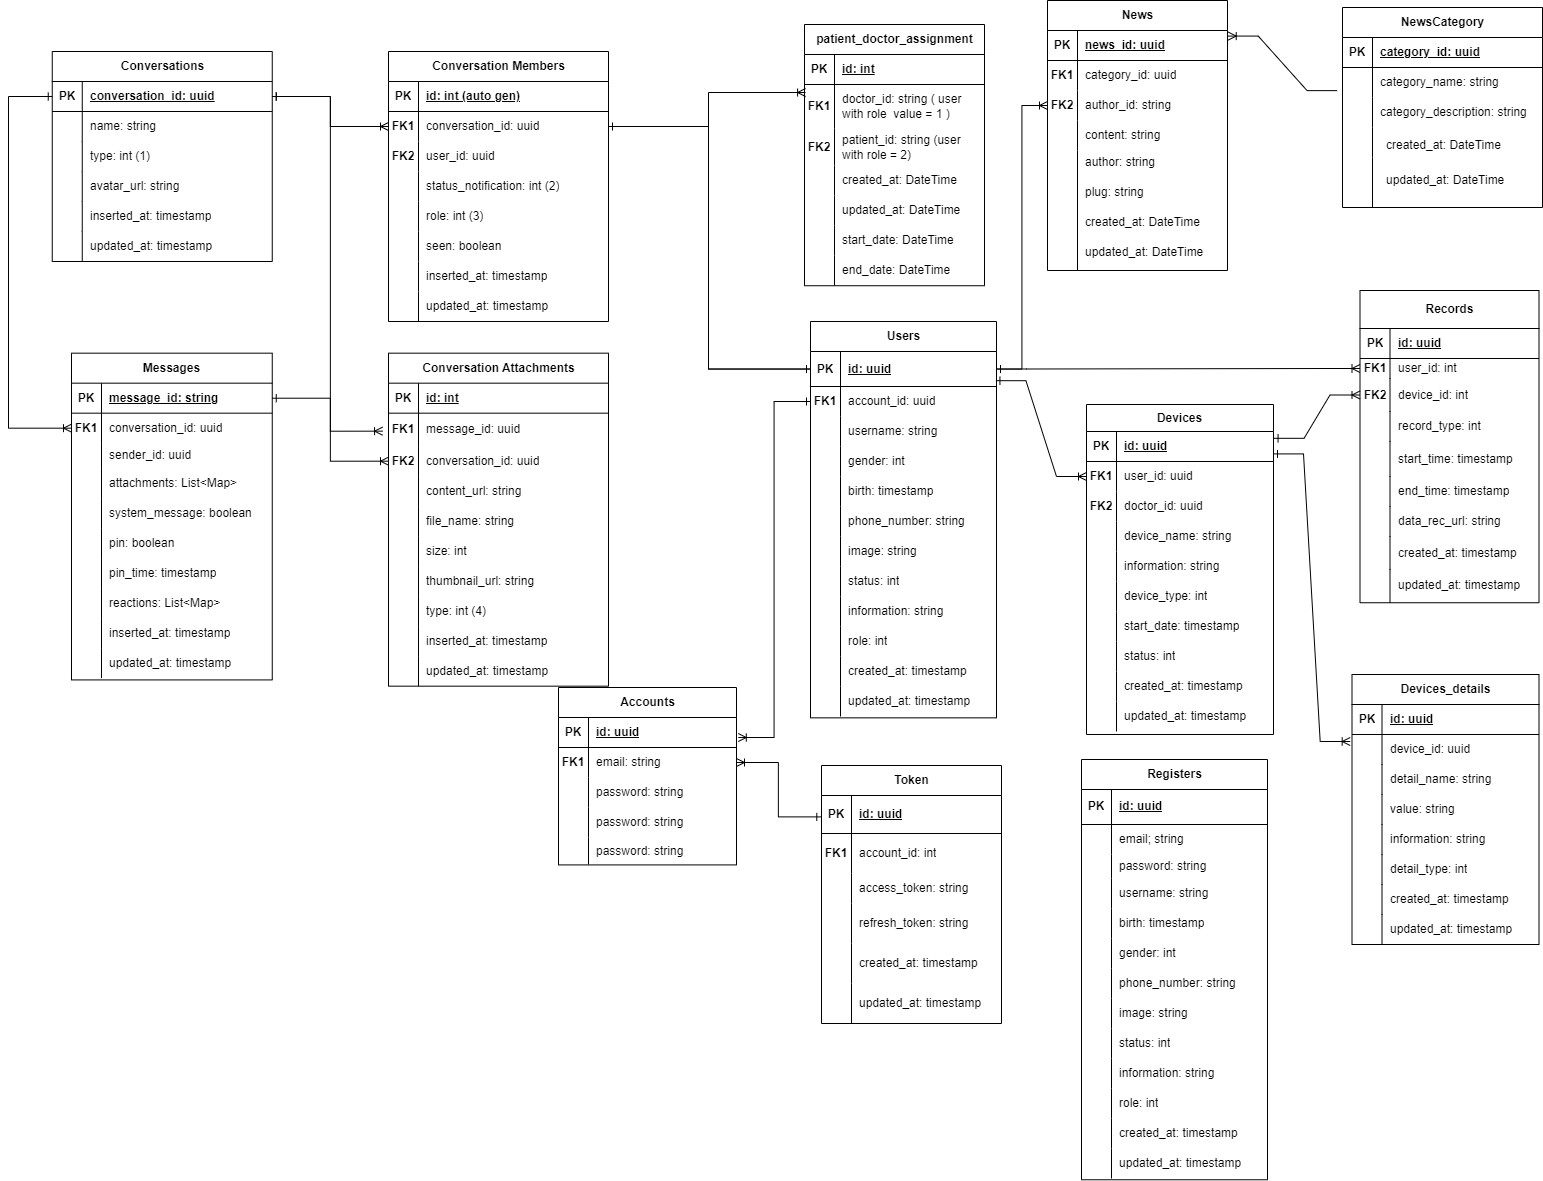
\includegraphics[width=15cm,height=15cm]{Images/system/fmECG_database.png}
	\caption[Sơ đồ ERD]{\bfseries \fontsize{12pt}{0pt}\selectfont Sơ đồ ERD}
	\label{fmECG_architecture-Database}
\end{figure}

\subsection{Thiết kế giao diện}

\subsection{Thiết kế các chức năng cho website và server}

\subsubsection{Thiết kế các API cần thiết}


\begin{enumerate}[a)]
	\item API xác minh tài khoản

	\begin{xltabular}{\textwidth}{
	  | >{\raggedright\arraybackslash}m{4.6cm}
	  | >{\centering\arraybackslash}m{2.8cm}
	  | >{\raggedright\arraybackslash}X |
	  }
	  \caption{\bfseries \fontsize{12pt}{0pt}\selectfont Bảng API xác minh tài khoản}
	  \label{table_api_auth}
	  \\
	  \hline
	  \bfseries Đường dẫn    &\bfseries Phương thức    &\bfseries Mô tả\\ \hline
	  api/ecg/auth/create-account   &   POST  & Tạo mới tài khoản người dùng \\ \hline
	  api/ecg/auth/login   &    POST    & Đăng nhập vào hệ thống \\ \hline
	  api/ecg/auth/logout   &    POST    & Đăng xuất khỏi hệ thống \\ \hline
	\end{xltabular}
  
	\item API quản lý người dùng trong hệ thống
	\begin{xltabular}{\textwidth}{
	  | >{\raggedright\arraybackslash}m{4.6cm}
	  | >{\centering\arraybackslash}m{2.8cm}
	  | >{\raggedright\arraybackslash}X |
	  }
	  \caption{\bfseries \fontsize{12pt}{0pt}\selectfont Bảng API quản lý người dùng trong hệ thống}
	  \label{table_api_user}
	  \\
	  \hline
	  \bfseries Đường dẫn    &\bfseries Phương thức    &\bfseries Mô tả\\ \hline
	  api/ecg/users   &   GET  &  Tra cứu danh sách tất cả người dùng trong hệ thống\\  \hline
	  api/ecg/users/doctors   &   GET  &  Tra cứu danh sách toàn bộ bác sĩ trong hệ thống \\  \hline
	  api/ecg/users/:id   &   GET  &  Tra cứu dữ liệu người dùng cụ thể dựa trên id tương ứng \\  \hline
	  api/ecg/users/data/patient-data   &   GET  &  Tra cứu danh sách các bệnh nhân đang được theo dõi của bác sĩ cụ thể \\  \hline
	  api/ecg/users/   &   PUT  &  Chỉnh sửa thông tin người dùng \\  \hline
	  api/ecg/users/:userId  &   DELETE  &  Xóa người dùng cụ thể dựa trên id tương ứng \\  \hline
	\end{xltabular}
  
  \item API quản lý thiết bị y tế
  \begin{xltabular}{\textwidth}{
	| >{\raggedright\arraybackslash}m{4.8cm}
	| >{\centering\arraybackslash}m{2.8cm}
	| >{\raggedright\arraybackslash}X |
	}
	\caption{\bfseries \fontsize{12pt}{0pt}\selectfont Bảng API quản lý thiết bị y tế}
	\label{table_api_device}
	\\
	\hline
	\bfseries Đường dẫn    &\bfseries Phương thức    &\bfseries Mô tả\\ \hline
	api/ecg/device   &   GET  & Tra cứu danh sách toàn bộ thiết bị y tế trong hệ thống\\ \hline
	api/ecg/devide/:id   &    GET    & Tra cứu thông tin chi tiết của một thiết bị y tế dựa trên id tương ứng \\ \hline
	api/ecg/device/add &   POST     & Thêm mới thiết bị y tế \\ \hline
	api/ecg/device-detail &   POST     & Thêm thông số kỹ thuật cho một thiết bị y tế \\ \hline
	api/ecg/device/:deviceId  &     PUT   & Cập nhật thông tin chi tiết cho thiết bị y tế cụ thể \\ \hline
	api/ecg/device/:deviceId  &     DELETE   & Xóa thiết bị y tế dựa trên id tương ứng \\ \hline
	api/ecg/device-detail  &     PUT   & Cập nhật thông số kỹ thuật cho thiết bị y tế \\ \hline
	api/ecg/device-detail/: detailId  &     PUT   & Xoá thông số kỹ thuật của thiết bị y tế \\ \hline
  \end{xltabular}
  
  \item API quản lý dữ liệu phiên đo
  \begin{xltabular}{\textwidth}{
	| >{\raggedright\arraybackslash}p{5cm}
	| >{\centering\arraybackslash}m{2.8cm}
	| >{\raggedright\arraybackslash}X |
	}
	\caption{\bfseries \fontsize{12pt}{0pt}\selectfont Bảng API quản lý dữ liệu phiên đo}
	\label{table_api_record}
	\\
	\hline
	\bfseries Đường dẫn    &\bfseries Phương thức    &\bfseries Mô tả \\ \hline
	 api/ecg/records   &   GET  & Tra cứu dữ liệu tất cả các phiên đo \\ \hline
	 api/ecg/records/:id   &    GET    & Tra cứu dữ liệu phiên đo cụ thể dựa theo id tương ứng \\ \hline
	 api/ecg/records/data/ doctorId &   GET     & Tra cứu dữ liệu tất cả các phiên đo của bệnh nhân mà bác sĩ phụ trách \\ \hline
	 api/ecg/records/   &    POST    & Tạo dữ liệu phiên đo mới \\ \hline
	 api/ecg/records/   &    PUT    & Cập nhật dữ liệu phiên đo \\ \hline
	 api/ecg/records/:recordId  &    DELETE    & Xóa dữ liệu phiên đo dựa theo id tương ứng \\ \hline
	\end{xltabular}
  
  
  \item API quản lý dịch vụ lịch khám
  \begin{xltabular}{\textwidth}{
	| >{\raggedright\arraybackslash}m{4.5cm}
	| >{\centering\arraybackslash}m{2.8cm}
	| >{\raggedright\arraybackslash}X |
	}
	\caption{\bfseries \fontsize{12pt}{0pt}\selectfont Bảng API quản lý dịch vụ lịch khám}
	\label{table_api_schedule}
	\\
	\hline
	\bfseries Đường dẫn    &\bfseries Phương thức    &\bfseries Mô tả\\ \hline
	api/ecg/schedules   &   GET  & Tra cứu danh sách tất cả lịch khám trong hệ thống \\ \hline
	api/ecg/schedules/ doctorId  &    GET    & Tra cứu danh sách lịch khám của bác sĩ cụ thể \\ \hline
	api/ecg/schedules/ patientId  &    GET    & Tra cứu danh sách lịch khám của bệnh nhân cụ thể \\ \hline
	api/ecg/schedules/create-by-doctor  &    POST    & Cho phép bác sĩ đặt lịch tái khám cho bệnh nhân \\ \hline
	api/ecg/schedules/create-by-patient  &    POST    & Cho phép bệnh nhân đặt lịch khám với bác sĩ \\ \hline
	api/ecg/schedules/time/ available-doctor/: schedule-time  &    GET    & Tra cứu danh sách các bác sĩ khả dụng theo thời gian đã chọn \\ \hline
	api/ecg/schedules/ available-schedule/:id  &    GET    & Tra cứu các khung giờ trống có thể đặt lịch với bác sĩ cụ thể. \\ \hline
	api/ecg/schedules/accept-schedule  &    PUT    & Chấp nhận lịch khám cụ thể \\ \hline
	api/ecg/schedules/reject-schedule/:id  &    DELETE    & Từ chối lịch khám cụ thể \\ \hline
	\end{xltabular}
  
  \item API liên quan đến chẩn đoán cho bệnh nhân
  \begin{xltabular}{\textwidth}{
	| >{\raggedright\arraybackslash}m{4.5cm}
	| >{\centering\arraybackslash}m{2.8cm}
	| >{\raggedright\arraybackslash}X |
	}
	\caption{\bfseries \fontsize{12pt}{0pt}\selectfont Bảng API liên quan đến chẩn đoán cho bệnh nhân}
	\label{table_api_diagnosis}
	\\
	\hline
	\bfseries Đường dẫn    &\bfseries Phương thức    &\bfseries Mô tả\\ \hline
	api/ecg/diagnosis   &   POST  & Tạo chẩn đoán mới cho bệnh nhân \\ \hline
	api/ecg/diagnosis/ schedule/:scheduleId   &   POST  & Tra cứu thông tin chẩn đoán dựa trên id lịch khám tương ứng\\ \hline
	api/ecg/diagnosis/update   &   POST  & Cập nhật thông tin chẩn đoán \\ \hline
	\end{xltabular}
  
  
  \item API liên quan đến thông báo về lịch khám
  \begin{xltabular}{\textwidth}{
	| >{\raggedright\arraybackslash}m{4.5cm}
	| >{\centering\arraybackslash}m{2.8cm}
	| >{\raggedright\arraybackslash}X |
	}
	\caption{\bfseries \fontsize{12pt}{0pt}\selectfont Bảng API liên quan đến thông báo về lịch khám}
	\label{table_api_notification}
	\\
	\hline
	\bfseries Đường dẫn    &\bfseries Phương thức    &\bfseries Mô tả\\ \hline
	api/ecg/notification/get   &   GET  & Tra cứu tất cả các thông báo của người dùng cụ thể  \\ \hline
	api/ecg/notification   &   POST  & Tạo thông báo mới liên quan đến lịch khám \\ \hline
	api/ecg/notification/ update-seen   &   POST  & Cập nhật trạng thái thông báo đã được xem\\ \hline
	api/ecg/notification/:id   &   DELETE  & Xóa thông báo dựa trên id tương ứng\\ \hline
	\end{xltabular}
  
  \item API liên quan đến tin nhắn
  \begin{xltabular}{\textwidth}{
	| >{\raggedright\arraybackslash}m{4.5cm}
	| >{\centering\arraybackslash}m{2.8cm}
	| >{\raggedright\arraybackslash}X |
	}
	\caption{\bfseries \fontsize{12pt}{0pt}\selectfont Bảng API liên quan đến tin nhắn}
	\label{table_api_chat}
	\\
	\hline
	\bfseries Đường dẫn    &\bfseries Phương thức    &\bfseries Mô tả\\ \hline
	api/ecg/groupChat   &   POST  & Tạo nhóm trò chuyện mới  \\ \hline
	api/ecg/groupChat   &   GET  & Tra cứu danh sách các nhóm trò chuyện của người dùng  \\ \hline
	api/ecg/chat/messages/: groupChatId   &   GET  & Tra cứu lịch sử trò chuyện của các đoạn hội thoại đã thực hiện \\ \hline
	api/ecg/chat/send   &   POST  & Cho phép người dùng gửi tin nhắn đến các đối tượng liên quan \\ \hline
	\end{xltabular}
\end{enumerate}


\subsubsection{Sơ đồ tuần tự API}
Phần này cung cấp các sơ đồ tuần tự minh họa chi tiết cách thức hoạt động của các API trong hệ thống.
Dựa trên bảng API đã thiết kế, các sơ đồ tuần tự sẽ mô phỏng luồng xử lý từ khi nhận yêu cầu đến khi trả về kết quả cho người dùng,
cho thấy rõ sự tương tác giữa các thành phần và lớp chức năng trong hệ thống.
% ------------------------Auth----------------------

\paragraph{Các API phục vụ mục đích xác minh tài khoản}
\mbox{}

\begin{figure}[H]
	\centering
	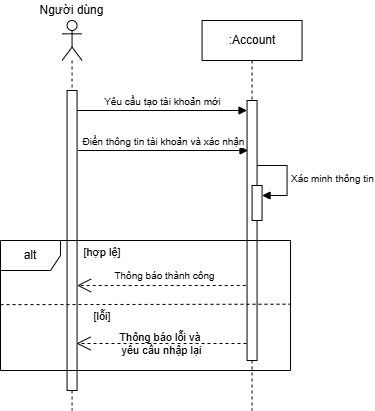
\includegraphics[width=15cm,height=15cm]{Images/sequence/user/register.drawio.png}
	\caption[Sơ đồ tuần tự API tạo mới tài khoản người dùng]{\bfseries \fontsize{12pt}{0pt}\selectfont Sơ đồ tuần tự API tạo mới tài khoản người dùng}
	\label{sequence_diagram_create_account}
\end{figure}

\begin{figure}[H]
	\centering
	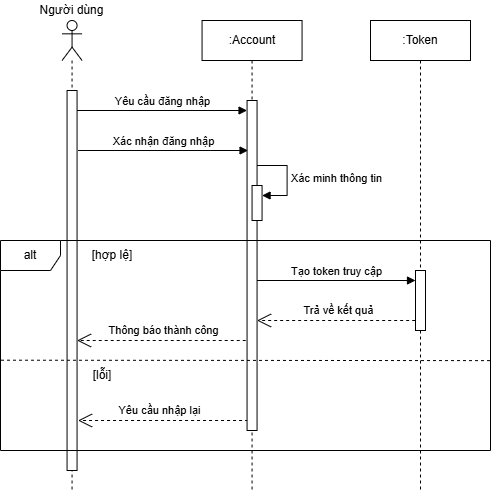
\includegraphics[width=15cm,height=15cm]{Images/sequence/user/login.drawio.png}
	\caption[Sơ đồ tuần tự API đăng nhập vào hệ thống]{\bfseries \fontsize{12pt}{0pt}\selectfont Sơ đồ tuần tự API đăng nhập vào hệ thống}
	\label{sequence_diagram_login}
\end{figure}

\begin{figure}[H]
	\centering
	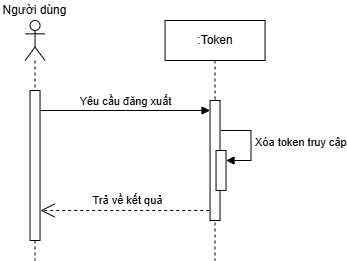
\includegraphics[width=13cm,height=10cm]{Images/sequence/user/logout.drawio.png}
	\caption[Sơ đồ tuần tự API đăng xuất khỏi hệ thống]{\bfseries \fontsize{12pt}{0pt}\selectfont Sơ đồ tuần tự API đăng xuất khỏi hệ thống}
	\label{sequence_diagram_logout}
\end{figure}

% % ------------------------User----------------------
\paragraph{Các API phục vụ mục đích quản lý người dùng trong hệ thống}
\mbox{}
\begin{figure}[H]
	\centering
	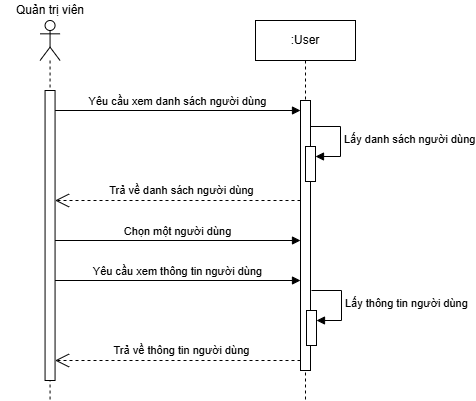
\includegraphics[width=15cm,height=15cm]{Images/sequence/user/getAllUser.drawio.png}
	\caption[Sơ đồ tuần tự API tra cứu danh sách tất cả người dùng trong hệ thống]{\bfseries \fontsize{12pt}{0pt}\selectfont Sơ đồ tuần tự API tra cứu danh sách tất cả người dùng trong hệ thống}
	\label{sequence_diagram_get_all_users}
\end{figure}

\begin{figure}[H]
	\centering
	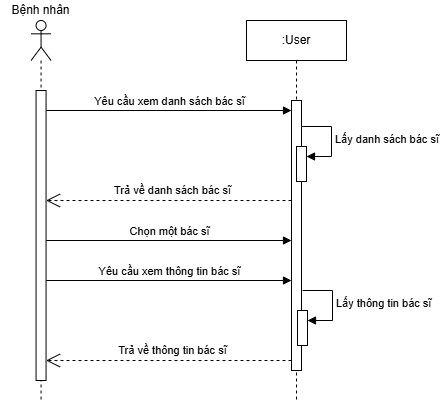
\includegraphics[width=15cm,height=15cm]{Images/sequence/user/getDoctor.drawio.png}
	\caption[Sơ đồ tuần tự API tra cứu danh sách toàn bộ bác sĩ trong hệ thống]{\bfseries \fontsize{12pt}{0pt}\selectfont Sơ đồ tuần tự API tra cứu danh sách toàn bộ bác sĩ trong hệ thống}
	\label{sequence_diagram_get_all_doctors}
\end{figure}

\begin{figure}[H]
	\centering
	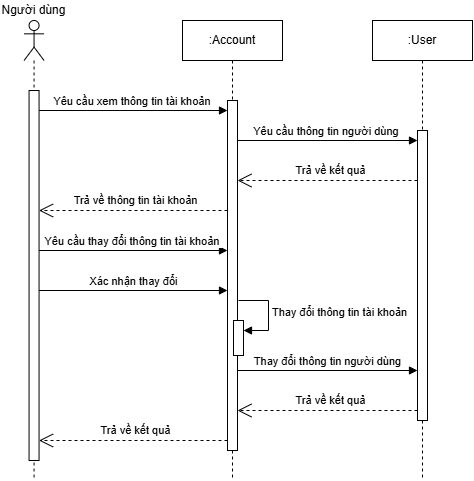
\includegraphics[width=16cm,height=14cm]{Images/sequence/user/account_info.drawio.png}
	\caption[Sơ đồ tuần tự API tra cứu dữ liệu người dùng cụ thể dựa trên id]{\bfseries \fontsize{12pt}{0pt}\selectfont Sơ đồ tuần tự API tra cứu dữ liệu người dùng cụ thể dựa trên id}
	\label{sequence_diagram_get_user_by_id}
\end{figure}

\begin{figure}[H]
	\centering
	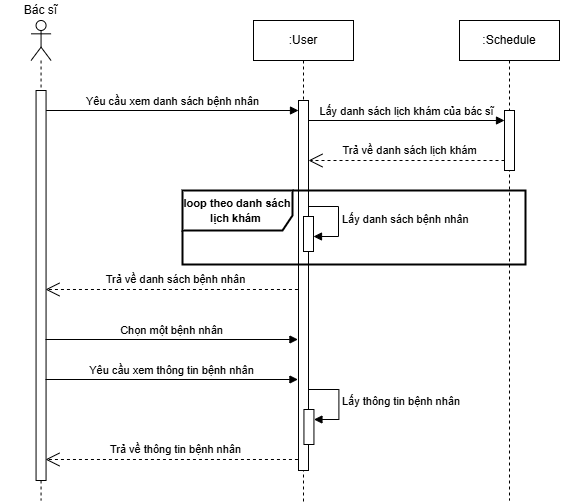
\includegraphics[width=15cm,height=15cm]{Images/sequence/user/getPatientByDoctor.drawio.png}
	\caption[Sơ đồ tuần tự API tra cứu danh sách bệnh nhân đang được theo dõi]{\bfseries \fontsize{12pt}{0pt}\selectfont Sơ đồ tuần tự API tra cứu danh sách bệnh nhân đang được theo dõi}
	\label{sequence_diagram_get_patient_data}
\end{figure}

\begin{figure}[H]
	\centering
	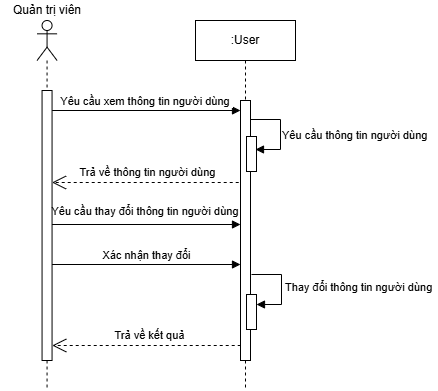
\includegraphics[width=15cm,height=15cm]{Images/sequence/user/update.drawio.png}
	\caption[Sơ đồ tuần tự API chỉnh sửa thông tin người dùng]{\bfseries \fontsize{12pt}{0pt}\selectfont Sơ đồ tuần tự API chỉnh sửa thông tin người dùng}
	\label{sequence_diagram_update_user}
\end{figure}

\begin{figure}[H]
	\centering
	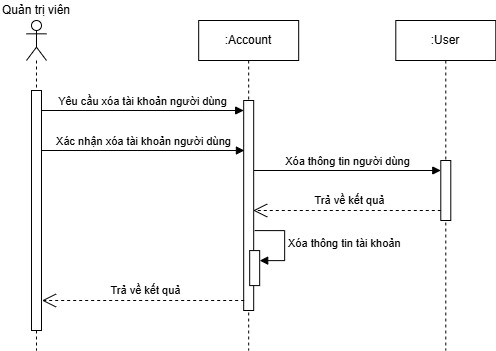
\includegraphics[width=15cm,height=15cm]{Images/sequence/user/delete.drawio.png}
	\caption[Sơ đồ tuần tự API xóa người dùng cụ thể dựa trên id]{\bfseries \fontsize{12pt}{0pt}\selectfont Sơ đồ tuần tự API xóa người dùng cụ thể dựa trên id}
	\label{sequence_diagram_delete_user}
\end{figure}

% % ------------------------Device----------------------
\paragraph{Các API phục vụ mục đích quản lý thiết bị y tế}
\mbox{}
\begin{figure}[H]
	\centering
	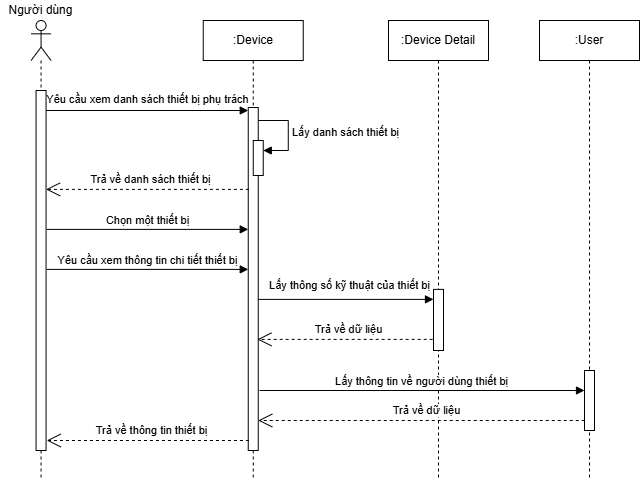
\includegraphics[width=15cm,height=15cm]{Images/sequence/device/getAll.drawio.png}
	\caption[Sơ đồ tuần tự API tra cứu danh sách thiết bị y tế]{\bfseries \fontsize{12pt}{0pt}\selectfont Sơ đồ tuần tự API tra cứu danh sách toàn bộ thiết bị y tế}
	\label{sequence_diagram_get_all_devices}
\end{figure}

\begin{figure}[H]
	\centering
	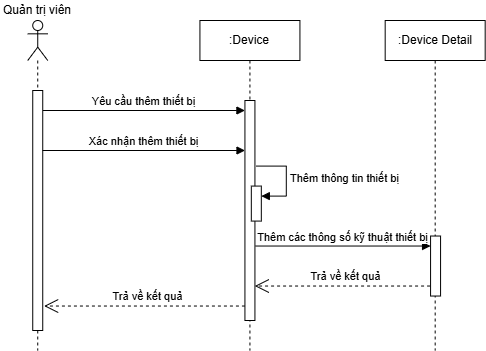
\includegraphics[width=15cm,height=15cm]{Images/sequence/device/add.drawio.png}
	\caption[Sơ đồ tuần tự API thêm mới thiết bị y tế]{\bfseries \fontsize{12pt}{0pt}\selectfont Sơ đồ tuần tự API thêm mới thiết bị y tế}
	\label{sequence_diagram_add_device}
\end{figure}

\begin{figure}[H]
	\centering
	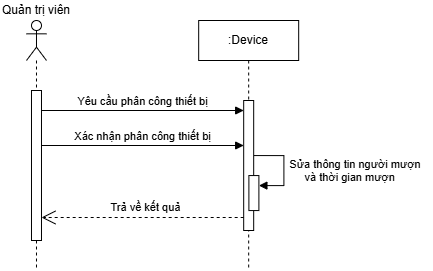
\includegraphics[width=15cm,height=11cm]{Images/sequence/device/assign.drawio.png}
	\caption[Sơ đồ tuần tự API đăng ký mượn thiết bị]{\bfseries \fontsize{12pt}{0pt}\selectfont Sơ đồ tuần tự API đăng ký mượn thiết bị}
	\label{sequence_diagram_add_device}
\end{figure}

\begin{figure}[H]
	\centering
	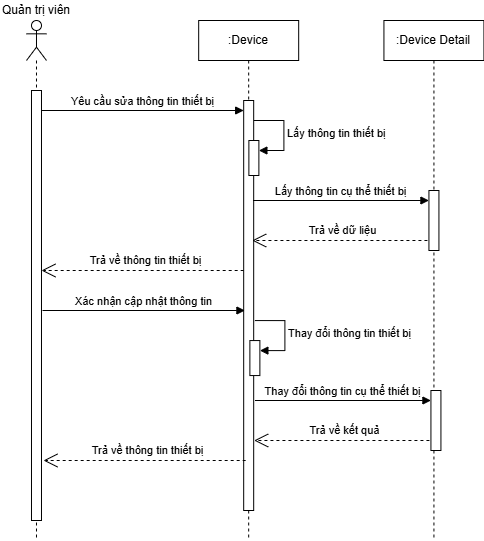
\includegraphics[width=15cm,height=15cm]{Images/sequence/device/update.drawio.png}
	\caption[Sơ đồ tuần tự API Cập nhật thiết bị và thông số kỹ thuật (nếu cần)]{\bfseries \fontsize{12pt}{0pt}\selectfont Sơ đồ tuần tự API Cập nhật thiết bị và thông số kỹ thuật (nếu cần)}
	\label{sequence_diagram_update_device}
\end{figure}

\begin{figure}[H]
	\centering
	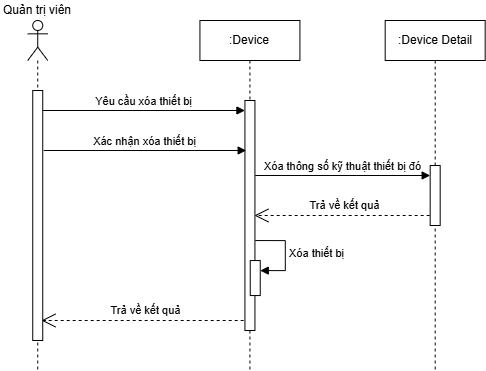
\includegraphics[width=15cm,height=13cm]{Images/sequence/device/delete.drawio.png}
	\caption[Sơ đồ tuần tự API xóa thiết bị y tế]{\bfseries \fontsize{12pt}{0pt}\selectfont Sơ đồ tuần tự API xóa thiết bị y tế}
	\label{sequence_diagram_get_device_by_id}
\end{figure}

% % ------------------------Schedule----------------------
\paragraph{Các API phục vụ mục đích đặt lịch hẹn bác sĩ - bệnh nhân}
\mbox{}
\begin{figure}[H]
	\centering
	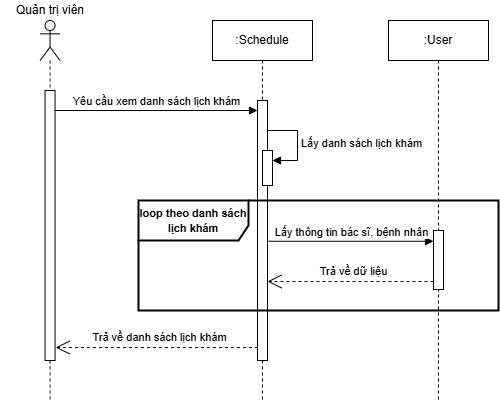
\includegraphics[width=15cm,height=15cm]{Images/sequence/schedule/getAll.drawio.png}
	\caption[Sơ đồ tuần tự API tra cứu tất cả lịch hẹn]{\bfseries \fontsize{12pt}{0pt}\selectfont Sơ đồ tuần tự API tra cứu tất cả lịch hẹn}
	\label{sequence_diagram_get_schedule}
\end{figure}

\begin{figure}[H]
	\centering
	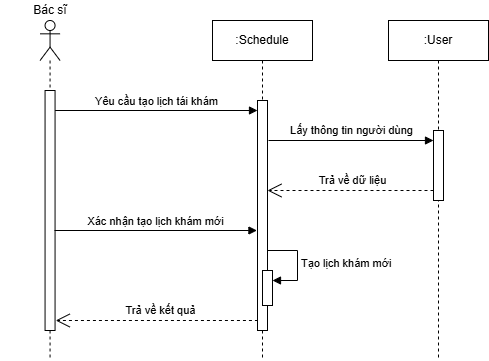
\includegraphics[width=15cm,height=15cm]{Images/sequence/schedule/createByDoctor.drawio.png}
	\caption[Sơ đồ tuần tự API bác sĩ tạo lịch tái khám cho bệnh nhân]{\bfseries \fontsize{12pt}{0pt}\selectfont Sơ đồ tuần tự API bác sĩ tạo lịch tái khám cho bệnh nhân}
	\label{sequence_diagram_create_schedule_by_doctor}
\end{figure}

\begin{figure}[H]
	\centering
	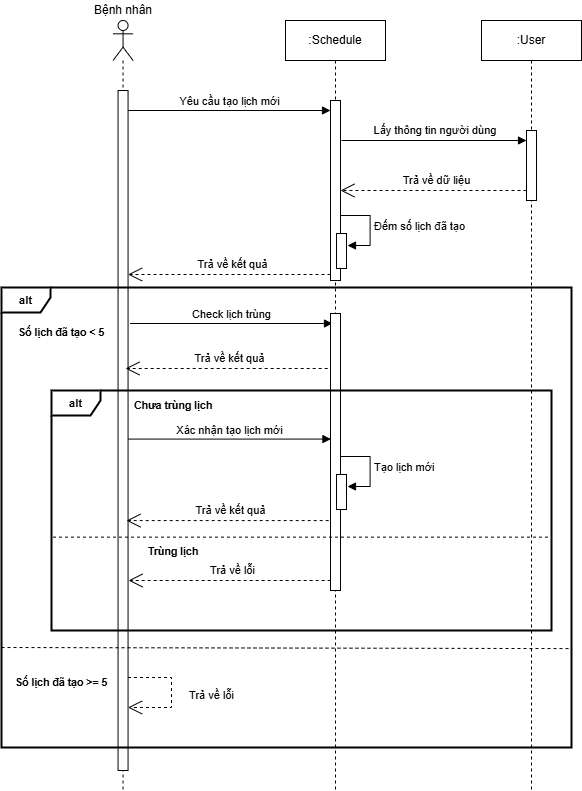
\includegraphics[width=15cm,height=15cm]{Images/sequence/schedule/createByPatient.drawio.png}
	\caption[Sơ đồ tuần tự API bệnh nhân chủ động đặt lịch hẹn]{\bfseries \fontsize{12pt}{0pt}\selectfont Sơ đồ tuần tự API bệnh nhân chủ động đặt lịch hẹn}
	\label{sequence_diagram_create_schedule_by_patient}
\end{figure}

\begin{figure}[H]
	\centering
	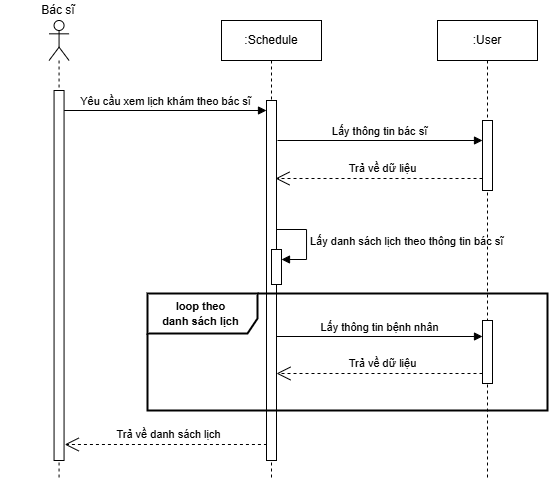
\includegraphics[width=15cm,height=15cm]{Images/sequence/schedule/getByDoctor.drawio.png}
	\caption[Sơ đồ tuần tự API tra cứu lịch hẹn của bác sĩ cụ thể]{\bfseries \fontsize{12pt}{0pt}\selectfont Sơ đồ tuần tự API tra cứu lịch hẹn của bác sĩ cụ thể}
	\label{sequence_diagram_get_schedule_by_doctor}
\end{figure}

\begin{figure}[H]
	\centering
	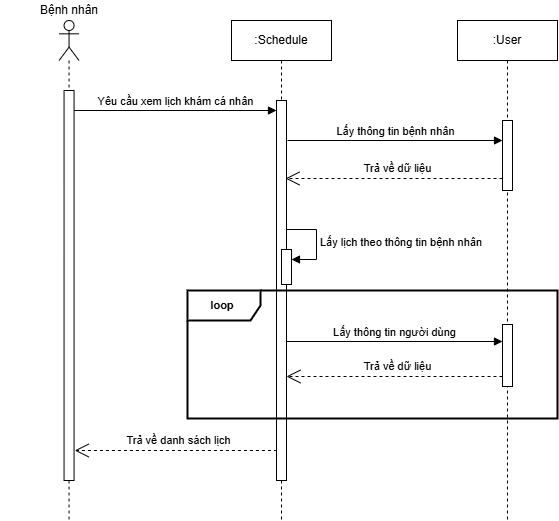
\includegraphics[width=15cm,height=15cm]{Images/sequence/schedule/getByPatient.drawio.png}
	\caption[Sơ đồ tuần tự API tra cứu lịch hẹn của bệnh nhân cụ thể]{\bfseries \fontsize{12pt}{0pt}\selectfont Sơ đồ tuần tự API tra cứu lịch hẹn của bệnh nhân cụ thể}
	\label{sequence_diagram_get_schedule_by_patient}
\end{figure}

\begin{figure}[H]
	\centering
	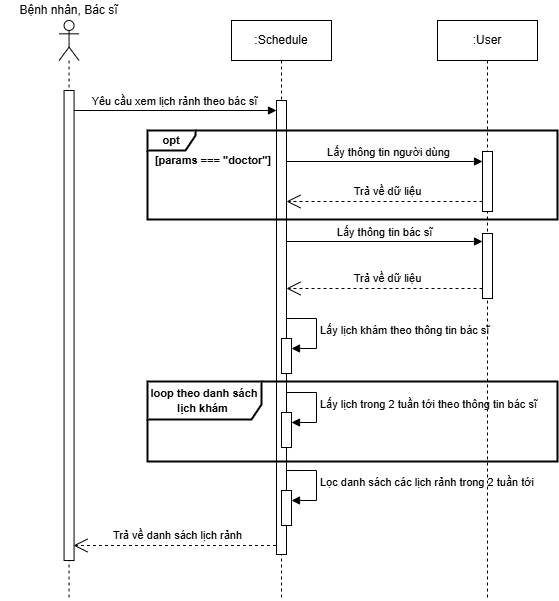
\includegraphics[width=15cm,height=15cm]{Images/sequence/schedule/getAvailableByDoctor.drawio.png}
	\caption[Sơ đồ tuần tự API tra cứu lịch rảnh của bác sĩ cụ thể]{\bfseries \fontsize{12pt}{0pt}\selectfont Sơ đồ tuần tự API tra cứu lịch rảnh của bác sĩ cụ thể}
	\label{sequence_diagram_get_available_by_doctor}
\end{figure}

\begin{figure}[H]
	\centering
	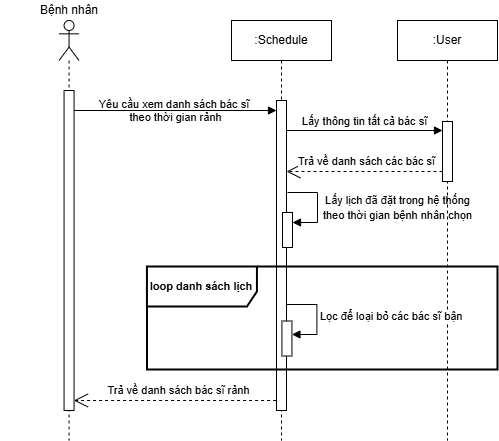
\includegraphics[width=15cm,height=15cm]{Images/sequence/schedule/getAvailableWithTime.drawio.png}
	\caption[Sơ đồ tuần tự API tra cứu bác sĩ phù hợp với thời gian đã chọn]{\bfseries \fontsize{12pt}{0pt}\selectfont Sơ đồ tuần tự API tra cứu bác sĩ phù hợp với thời gian đã chọn}
	\label{sequence_diagram_get_available_with_time}
\end{figure}

\begin{figure}[H]
	\centering
	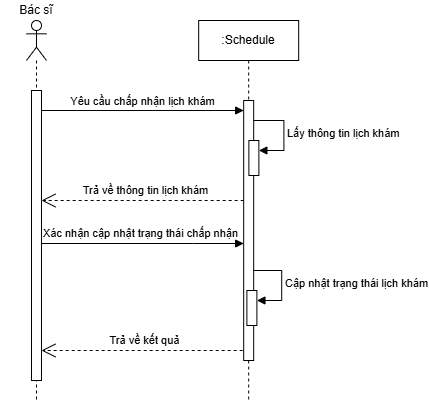
\includegraphics[width=15cm,height=15cm]{Images/sequence/schedule/accept.drawio.png}
	\caption[Sơ đồ tuần tự API bác sĩ xác nhận lịch hẹn]{\bfseries \fontsize{12pt}{0pt}\selectfont Sơ đồ tuần tự API bác sĩ xác nhận lịch hẹn}
	\label{sequence_diagram_accept_schedule}
\end{figure}

\begin{figure}[H]
	\centering
	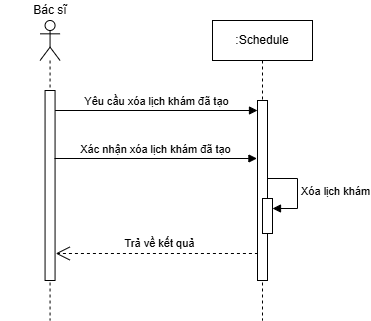
\includegraphics[width=10cm,height=9cm]{Images/sequence/schedule/delete.drawio.png}
	\caption[Sơ đồ tuần tự API bác sĩ từ chối lịch hẹn]{\bfseries \fontsize{12pt}{0pt}\selectfont Sơ đồ tuần tự API bác sĩ từ chối lịch hẹn}
	\label{sequence_diagram_reject_schedule}
\end{figure}
% % ------------------------Record----------------------
\paragraph{Các API phục vụ mục đích liên quan đến dữ liệu phiên đo}
\mbox{}
\begin{figure}[H]
	\centering
	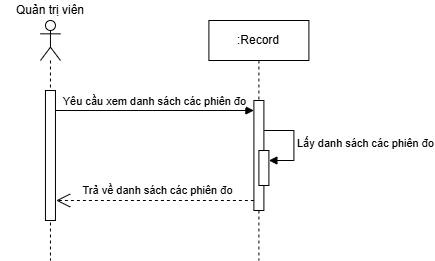
\includegraphics[width=11cm,height=9cm]{Images/sequence/record/getAll.drawio.png}
	\caption[Sơ đồ tuần tự API tra cứu danh sách các dữ liệu phiên đo]{\bfseries \fontsize{12pt}{0pt}\selectfont Sơ đồ tuần tự API tra cứu danh sách các dữ liệu phiên đo}
	\label{sequence_diagram_get_all_records}
\end{figure}

\begin{figure}[H]
	\centering
	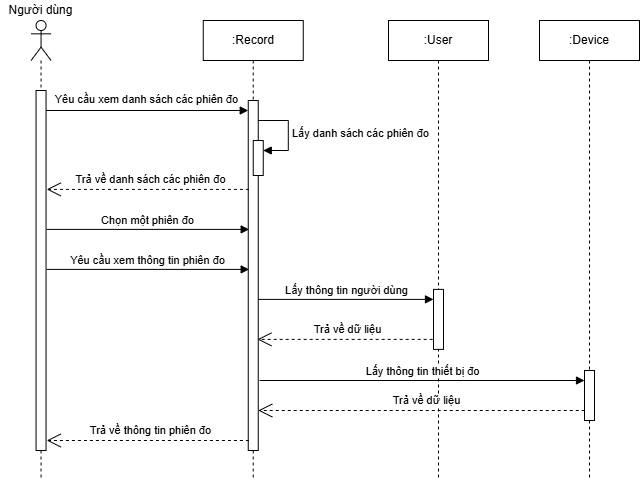
\includegraphics[width=15cm,height=15cm]{Images/sequence/record/getById.drawio.png}
	\caption[Sơ đồ tuần tự API tra cứu dữ liệu phiên đo theo id]{\bfseries \fontsize{12pt}{0pt}\selectfont Sơ đồ tuần tự API tra cứu dữ liệu phiên đo theo id}
	\label{sequence_diagram_get_record_by_id}
\end{figure}

\begin{figure}[H]
	\centering
	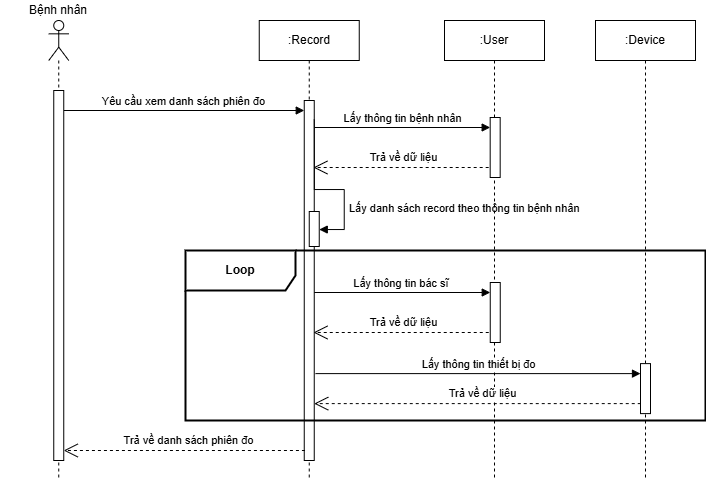
\includegraphics[width=15cm,height=15cm]{Images/sequence/record/getByPatientId.drawio.png}
	\caption[Sơ đồ tuần tự API tra cứu dữ liệu phiên đo của bệnh nhân]{\bfseries \fontsize{12pt}{0pt}\selectfont Sơ đồ tuần tự API tra cứu dữ liệu phiên đo của bệnh nhân}
	\label{sequence_diagram_get_record_by_patient_id}
\end{figure}

\begin{figure}[H]
	\centering
	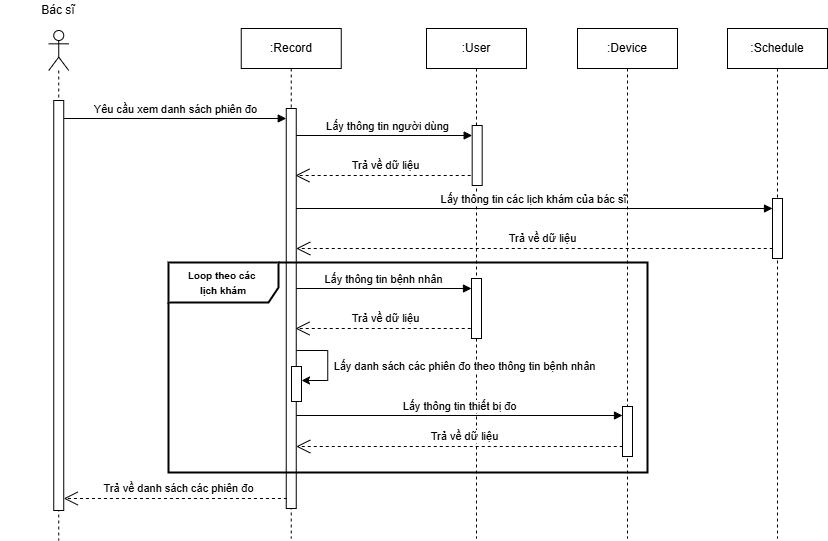
\includegraphics[width=15cm,height=15cm]{Images/sequence/record/getByDoctorId.drawio.png}
	\caption[Sơ đồ tuần tự API tra cứu dữ liệu phiên đo do bác sĩ phụ trách]{\bfseries \fontsize{12pt}{0pt}\selectfont Sơ đồ tuần tự API tra cứu dữ liệu phiên đo do bác sĩ phụ trách}
	\label{sequence_diagram_get_record_by_doctor_id}
\end{figure}

\begin{figure}[H]
	\centering
	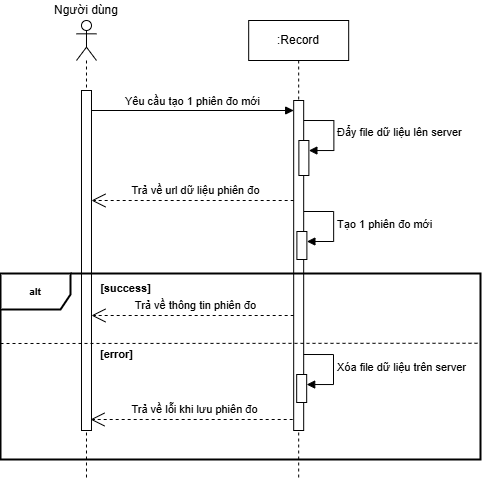
\includegraphics[width=15cm,height=15cm]{Images/sequence/record/create.drawio.png}
	\caption[Sơ đồ tuần tự API tạo mới dữ liệu phiên đo]{\bfseries \fontsize{12pt}{0pt}\selectfont Sơ đồ tuần tự API tạo mới dữ liệu phiên đo}
	\label{sequence_diagram_create_record}
\end{figure}

\begin{figure}[H]
	\centering
	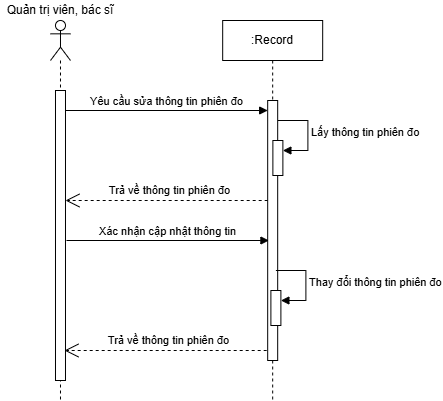
\includegraphics[width=15cm,height=15cm]{Images/sequence/record/update.drawio.png}
	\caption[Sơ đồ tuần tự API cập nhật dữ liệu phiên đo]{\bfseries \fontsize{12pt}{0pt}\selectfont Sơ đồ tuần tự API cập nhật dữ liệu phiên đo}
	\label{sequence_diagram_update_record}
\end{figure}

\begin{figure}[H]
	\centering
	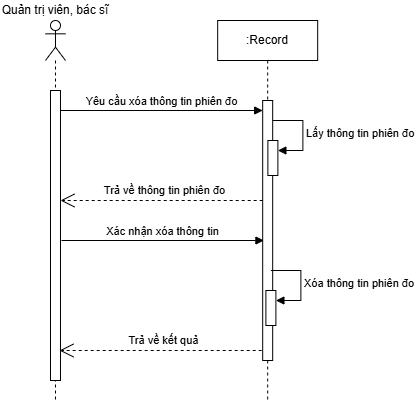
\includegraphics[width=15cm,height=15cm]{Images/sequence/record/delete.drawio.png}
	\caption[Sơ đồ tuần tự API xóa dữ liệu phiên đo]{\bfseries \fontsize{12pt}{0pt}\selectfont Sơ đồ tuần tự API xóa dữ liệu phiên đo}
	\label{sequence_diagram_delete_record}
\end{figure}

\begin{figure}[H]
	\centering
	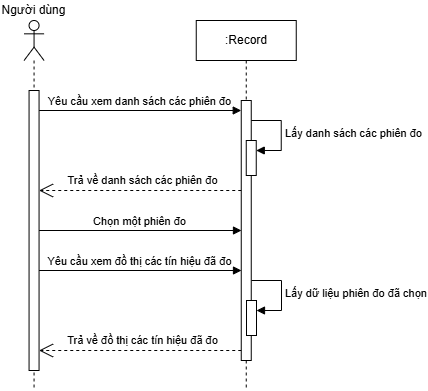
\includegraphics[width=15cm,height=15cm]{Images/sequence/record/chart.drawio.png}
	\caption[Sơ đồ tuần tự API tra cứu đồ thị các tín hiệu đã đo]{\bfseries \fontsize{12pt}{0pt}\selectfont Sơ đồ tuần tự API tra cứu đồ thị các tín hiệu đã đo}
	\label{sequence_diagram_chart_record}
\end{figure}
% % ------------------------Diag----------------------
\paragraph{Các API phục vụ mục đích liên quan đến chẩn đoán}
\mbox{}

\begin{figure}[H]
	\centering
	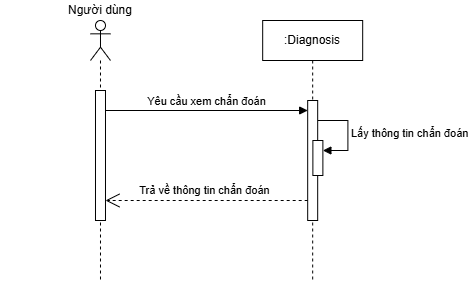
\includegraphics[width=15cm,height=11cm]{Images/sequence/diagnosis/getByScheduleId.drawio.png}
	\caption[Sơ đồ tuần tự API lấy chẩn đoán theo lịch hẹn]{\bfseries \fontsize{12pt}{0pt}\selectfont Sơ đồ tuần tự API lấy chẩn đoán theo lịch hẹn}
	\label{sequence_diagram_get_diagnosis_by_schedule}
\end{figure}

\begin{figure}[H]
	\centering
	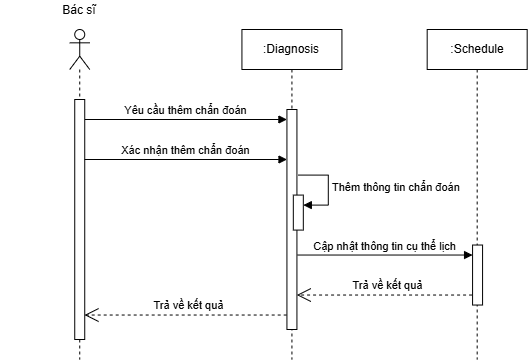
\includegraphics[width=15cm,height=12cm]{Images/sequence/diagnosis/create.drawio.png}
	\caption[Sơ đồ tuần tự API tạo mới chẩn đoán]{\bfseries \fontsize{12pt}{0pt}\selectfont Sơ đồ tuần tự API tạo mới chẩn đoán}
	\label{sequence_diagram_create_diagnosis}
\end{figure}

\begin{figure}[H]
	\centering
	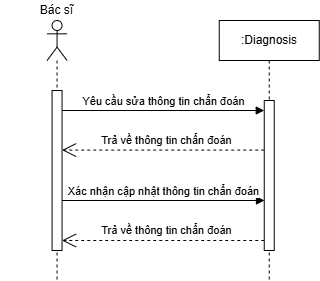
\includegraphics[width=15cm,height=11cm]{Images/sequence/diagnosis/update.drawio.png}
	\caption[Sơ đồ tuần tự API cập nhật thông tin chẩn đoán]{\bfseries \fontsize{12pt}{0pt}\selectfont Sơ đồ tuần tự API cập nhật thông tin chẩn đoán}
	\label{sequence_diagram_update_diagnosis}
\end{figure}
% % ------------------------Noti----------------------
\paragraph{Các API phục vụ mục đích liên quan đến thông báo}
\mbox{}
\begin{figure}[H]
	\centering
	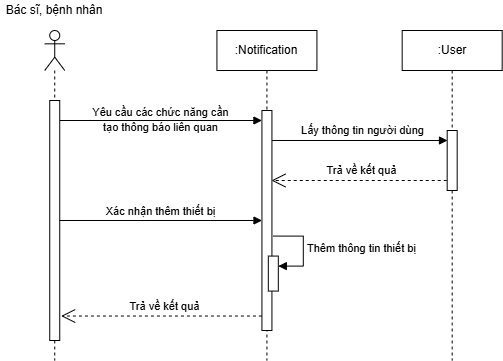
\includegraphics[width=15cm,height=12cm]{Images/sequence/notification/create.drawio.png}
	\caption[Sơ đồ tuần tự API tạo thông báo mới]{\bfseries \fontsize{12pt}{0pt}\selectfont Sơ đồ tuần tự API tạo thông báo mới}
	\label{sequence_diagram_create_notification}
\end{figure}

\begin{figure}[H]
	\centering
	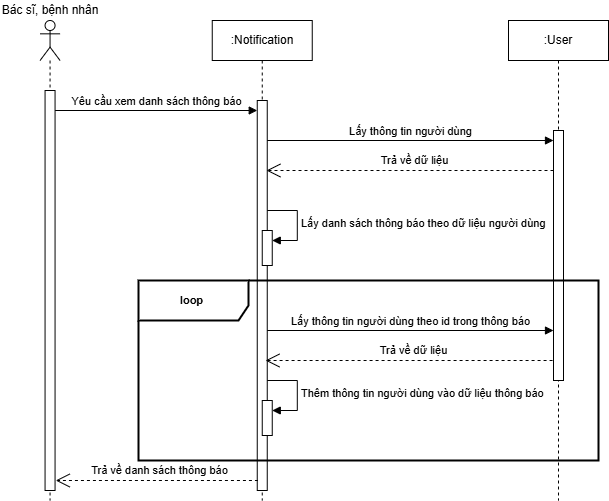
\includegraphics[width=15cm,height=15cm]{Images/sequence/notification/getByUserId.drawio.png}
	\caption[Sơ đồ tuần tự API lấy danh sách thông báo của người dùng]{\bfseries \fontsize{12pt}{0pt}\selectfont Sơ đồ tuần tự API lấy danh sách thông báo của người dùng}
	\label{sequence_diagram_get_notification_by_user}
\end{figure}

\begin{figure}[H]
	\centering
	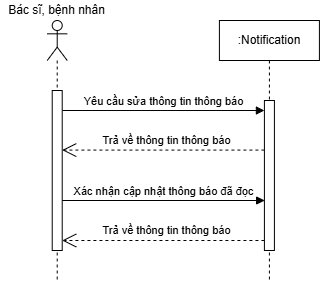
\includegraphics[width=8cm,height=8cm]{Images/sequence/notification/updateSeen.drawio.png}
	\caption[Sơ đồ tuần tự API cập nhật trạng thái đã xem thông báo]{\bfseries \fontsize{12pt}{0pt}\selectfont Sơ đồ tuần tự API cập nhật trạng thái đã xem thông báo}
	\label{sequence_diagram_update_seen}
\end{figure}

\begin{figure}[H]
	\centering
	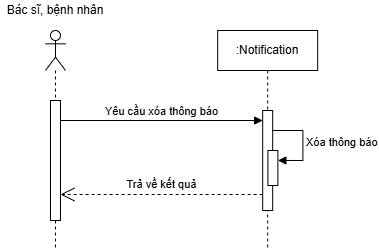
\includegraphics[width=15cm,height=11cm]{Images/sequence/notification/delete.drawio.png}
	\caption[Sơ đồ tuần tự API xóa thông báo]{\bfseries \fontsize{12pt}{0pt}\selectfont Sơ đồ tuần tự API xóa thông báo}
	\label{sequence_diagram_delete_notification}
\end{figure}
% % ------------------------Chat----------------------
\paragraph{Các API phục vụ mục đích liên quan đến tin nhắn}
\mbox{}
\begin{figure}[H]
	\centering
	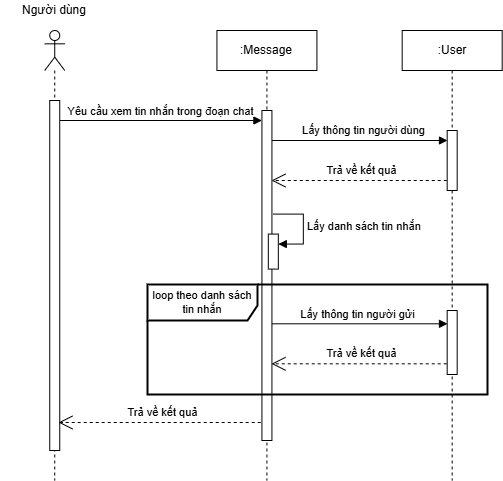
\includegraphics[width=15cm,height=15cm]{Images/sequence/chat/load.drawio.png}
	\caption[Sơ đồ tuần tự API lấy danh sách tin nhắn của người dùng]{\bfseries \fontsize{12pt}{0pt}\selectfont Sơ đồ tuần tự API lấy danh sách tin nhắn của người dùng}
	\label{sequence_diagram_load_chat}
\end{figure}

\begin{figure}[H]
	\centering
	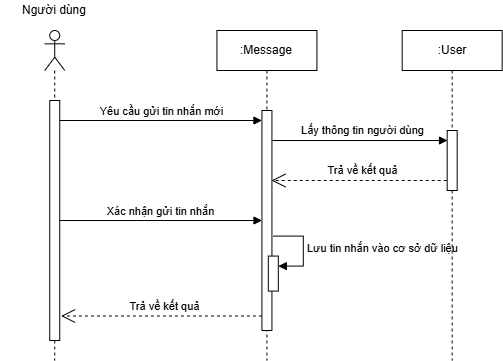
\includegraphics[width=15cm,height=12cm]{Images/sequence/chat/send.drawio.png}
	\caption[Sơ đồ tuần tự API gửi tin nhắn trong nhóm trò chuyện]{\bfseries \fontsize{12pt}{0pt}\selectfont Sơ đồ tuần tự API gửi tin nhắn trong nhóm trò chuyện}
	\label{sequence_diagram_send_chat}
\end{figure}

\begin{figure}[H]
	\centering
	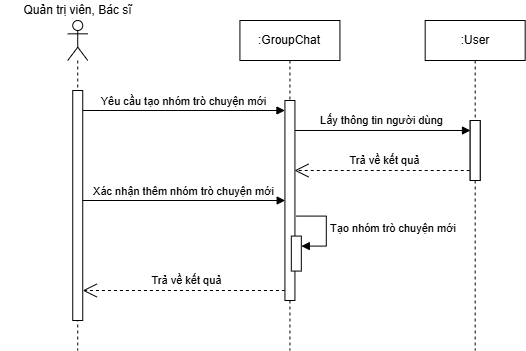
\includegraphics[width=15cm,height=12cm]{Images/sequence/chat/createGroupChat.drawio.png}
	\caption[Sơ đồ tuần tự API tạo nhóm trò chuyện mới]{\bfseries \fontsize{12pt}{0pt}\selectfont Sơ đồ tuần tự API tạo nhóm trò chuyện mới}
	\label{sequence_diagram_create_group_chat}
\end{figure}

\begin{figure}[H]
	\centering
	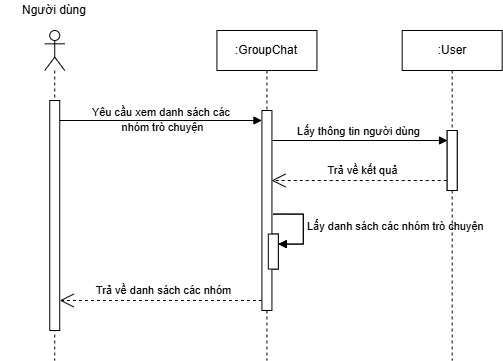
\includegraphics[width=15cm,height=12cm]{Images/sequence/chat/getGroupChat.drawio.png}
	\caption[Sơ đồ tuần tự API lấy danh sách nhóm trò chuyện của người dùng]{\bfseries \fontsize{12pt}{0pt}\selectfont Sơ đồ tuần tự API lấy danh sách nhóm trò chuyện của người dùng}
	\label{sequence_diagram_get_group_chat}
\end{figure}
\subsection{Kết luận chương}

Chương 3 trình bày chi tiết về quá trình thiết kế hệ thống, bao gồm kiến trúc tổng thể và các thành phần cụ thể.
Thiết kế hệ thống tập trung vào việc xây dựng kiến trúc vận hành hiệu quả và mượt mà, chú trọng vào tính bảo mật, hiệu suất và khả năng mở rộng tối ưu.
\newpage